\documentclass[a4paper,12pt,openany]{report}
\usepackage[left=4cm,right=2.5cm,top=4cm,bottom=2.5cm]{geometry}
\usepackage{physics}
\usepackage[spanish]{babel}
\usepackage[utf8x]{inputenc}
\usepackage{amsfonts,amssymb,amsmath,amsthm}
\usepackage{txfonts}
\usepackage{subcaption}
\usepackage[colorlinks]{hyperref}
\usepackage{dsfont}
\usepackage[pdftex]{graphicx}
\usepackage{tocloft}

\setlength{\parskip}{0.4cm}

\newtheorem{theorem}{Teorema}
\newtheorem{lemma}[theorem]{Lema}

\newcommand{\cd}[1]{
\frac{\delta #1}{\mathrm{d}s}
}

\newcommand{\s}{									
\mathrm{s}
}

\newcommand{\des}[2]{
\stackrel{#1}{#2}{\!}
}

\newcommand{\dual}[1]{
{}^*\! #1
}

\begin{document}
\pagenumbering{roman}
\pagestyle{empty}
\thispagestyle{empty}
\pagestyle{empty}
\begin{center}
	\includegraphics[width=2cm]{logo_udec}\\
	\vspace{0.3cm}
	\textbf{UNIVERSIDAD DE CONCEPCI\'ON} \\ 
	\textbf{FACULTAD DE CIENCIAS F\'ISICAS Y MATEM\'ATICAS} \\
	\vspace{0.6cm}	
	\rule{14.5cm}{0.1cm}
	\vspace{0.5cm}

	
	{\Large \textbf{Analogía gravito-electromagnética basada en tensores de marea: órbitas helicoidales en la métrica de Kerr}}
	
	\vspace{1.0cm}
	
	{ Profesor Gu\'ia: \textbf{Dr. Guillermo Rubilar}\\ 
		Departamento de F\'isica \\ 
		Facultad de Ciencias F\'isicas y Matem\'aticas \\
		Universidad de Concepci\'on}
	
	\vspace{0.7cm}
	\rule{14.5cm}{0.1cm}
	\vspace{0.35cm}	
	
	
\textbf{Tesis presentada en la Facultad de Ciencias F\'isicas y Matem\'aticas para optar al grado de Mag\'ister en Ciencias con menci\'on en F\'isica\\
de la Universidad de Concepci\'on}

C\'odigo Programa: 4102
	\vfill
	por
	
	\textbf{Antonio Gonz\'alez Guerra \\ 
	CONCEPCI\'ON -  CHILE \\
	Junio 2019}
\end{center}

\thispagestyle{empty} 
\newpage

\pagestyle{myheadings}
\ \\
\vspace{10cm}
\vfill
\hspace{2.5cm}
\begin{tabular}[c]{lll}
	\ Comisi\'on examinadora & : & Dr. Guillermo Rubilar A. (gu\'ia)
	\bigskip
	\\
	\large & &  Dr. Julio Oliva Z. \\ \\
	& & Dr. Esteban Sep\'ulveda G.\\ \\
\end{tabular}
\thispagestyle{empty}

\pagestyle{myheadings}

\newpage
\thispagestyle{empty}
\textit{
Esta tesis ha sido escrita principalmente por A. Gonz\'alez con ayuda de G. Rubilar como fin de los trabajos realizados en pregrado y postgrado entre los anos 2016-2019, en la Universidad de Concepci\'on.}

\textit{
Los c\'odigos \LaTeX, como las figuras editables y los c\'odigos Python utilizados en esta tesis se encuentran disponibles en los repositorios GitHub de la tesis.
}

\textit{
\url{https://github.com/antongonzalez/tesis-magister.git}
}
\vspace*{\fill}
\begin{flushright}
\large
\textit{``Peter Parker... brilliant but lazy...''}

\footnotesize
- Si no sabes qui\'en lo dijo, creo que hay algo que debes hacer antes de leer esta tesis.
\end{flushright}

\newpage
\pagenumbering{Roman}
\chapter*{Agradecimientos}

Quisiera agradecer a mis padres por su apoyo durante mi gran proceso de formación en la Universidad y por haberme brindado la oportunidad de dedicar mi tiempo en una profesión que me apasiona y me hace feliz. 

Así mismo, también deseo agradecer al Dr. Guillermo Rubilar por su gran apoyo en sus cursos de formación y guía durante mi estancia en el postgrado, como al Dr. Joaquín Díaz de Valdés por su gran ayuda durante mi estancia en la facultad de Física. De igual forma, deseo agradecer al departamento de Física de la Universidad de Concepción y al Instituto Sudamericano de Investigaciones Fundamentales (ICTP-SAIFR) por darme la oportunidad de asistir a la escuela \textit{``The Sound of Space-time: The Dawn of Gravitational Wave Science''}, como a las personas que compartieron conmigo durante dicho evento.

Por último doy gracias a todas las personas que han compartido conmigo a lo largo de mis años de estudio, en especial a mis compañeros de carrera y oficina.

\newpage
\tableofcontents
\addtocontents{toc}{~\hfill\textbf{P\'agina}\par}

\newpage	
\phantomsection	
\addcontentsline{toc}{chapter}{Lista de figuras}
\listoffigures

\newpage
\addcontentsline{toc}{chapter}{Resumen}
\chapter*{Resumen}

En la presente se estudia una analogía propuesta, basada en tensores de marea, entre la teoría electromagnética clásica y la teoría de Relatividad General. Para esto se presentan ambas teorías de una forma compacta a modo de introducción, luego se utiliza la expansión multipolar para obtener las ecuaciones de movimiento **de que?** y luego compararlas usando **los tensores de marea a orden dipolar y cuadrupolar**. **Se analizan orbitas circulares en la metrica de kerr para el caso dipolar**.

 Por último se logra obtener una solución a las ecuaciones de movimiento para una un satélite con rotación intrínseca realizando una órbita circular al rededor de un agujero negro rotante.  Con el fin de estudiar las consecuencias del espín.
\newpage
\addcontentsline{toc}{chapter}{Introducci\'on}
\chapter*{Introducci\'on}

En la presente se estudia una analogía propuesta, basada en tensores de marea, entre la teoría electromagnética clásica y la teoría de Relatividad General. En \cite{Costa-Herdeiro} se plantea una nueva forma de establecer una relación entre la teoría de Relatividad General  y la teoría electromagnética clásica. A partir de los tensores de marea, los cuales permiten el estudio de las inhomogeneidades de los campos en cuestión, es se logra obtener una completa correspondencia entre los términos que describen el movimiento de un dipolo magnético y una partícula con espín \cite{Steinhoff-Puetzfeld}.

Para poder entender lo anterior de una forma más clara, en el capítulo \ref{cap:1} se introducen los temas relacionados con la teoría electromagnética clásica \cite{gr2}, desde las ecuaciones de Maxwell (y su respectiva formulación covariante), la obtención de la ecuación de desvío para un par de carga de prueba, finalizando con la expansión multipolar \cite{Dixon1,Dixon2,Dixon3} y el estudio del caso particular para un dipolo magnético.

Luego, en el capítulo \ref{cap:2} se introducen los distintos elementos de Relatividad General \cite{gr1,inverno,Steven,Hans,Poisson} desde presentar las ecuaciones de campo de Einstein, explicando el principio de equivalencia y describiendo la solución de Kerr \cite{Heinicke}, para después obtener la ecuación de desvío geodésico, y finalizando con la expansión multipolar gravitacional hasta orden cuadrupolar.

Habiendo resumido ambas teorías en los capítulos anteriores, en el capítulo \ref{cap:3} se presenta en detalle la analogía propuesta en \cite{Costa-Herdeiro}, para luego hacer uso de las ecuaciones de desvío obtenidas anteriormente para definir los tensores de marea electromagnéticos y gravitacionales, los cuales permitirán comparar ambas teorías. Luego, se hace una primera comparación estudiando campos gravitacionales débiles haciendo uso de teoría de perturbaciones. Y para finalizar, se estudian extensiones a la correspondencia existente para el caso dipolar en las ecuaciones de movimiento en ambos contextos, para luego realizar una discusión sobre las similitudes y diferencias entre la teoría de Relatividad General y la teoría electromagnética clásica.

Por último, en el capítulo \ref{cap:4} se estudia un caso particular en donde al considerar una 4-velocidad de la forma $u^{\mu}=\left[ u^t, 0, 0, u^{\phi} \right]$, se simplifican las ecuaciones de movimiento al punto de que es posible obtener soluciones analíticas. Este análisis surge por estudiar el análogo gravitacional de un problema presentado en \cite{Costa-Natario-Zilhao}, donde se puede hacer una simplificación similar considerando la misma 4-velocidad.
\newpage
\pagenumbering{arabic}
\chapter{Electrodinámica}
\label{cap:1}
\newpage

\section{Ecuaciones de Maxwell}

Desde el siglo XVIII diversos científicos de la época formularon leyes que permitían entender las diversas interacciones entre los campos eléctricos y magnéticos, entre las cuales destacan la \textit{ley de Coulomb}, la \textit{ley de Ampère}, la \textit{ley de Faraday} y la \textit{ley de Gauss}, entre otras. 

No fue hasta el año 1865 donde el físico James Clerk Maxwell (1831-1879) en su trabajo titulado \textit{A Dynamical Theory of the Electromagnetic Field} \cite{Maxwell} resume todas las leyes anteriormente nombradas a partir elementos más fundamentales logrando así toda la teoría electromagnética utilizando un conjunto de cuatro ecuaciones las cuales son (ver Apéndice \ref{ape:convenciones} para unidades):
\begin{center}
\begin{tabular}{l|c|c}
Nombre & Forma integral & Forma diferencial \\
\hline \hline
 & & \\
ley de Gauss & $\oiiint_{\partial \Omega} \vb{E} \cdot \mathrm{d}\vb{S} = \iiint_{\Omega} \rho \mathrm{d}V $ & $\div{\vb{E}} = 4\pi \rho$ \\
 & & \\
\hline
 & & \\
ley de Gauss magnética & $\oiiint_{\partial \Omega} \vb{B} \cdot \mathrm{d}\vb{S} = 0 $ & $\div{\vb{B}} = 0$ \\
 & & \\
\hline
 & & \\
ley de Faraday & $\oint_{\partial \Sigma} \vb{E} \cdot \mathrm{d} \vb{l} = - \pdv{}{t} \iint_{\Sigma} \vb{B} \cdot \mathrm{d} \vb{S}$ & $\curl{\vb{E}} = - \pdv{\vb{B}}{t}$ \\
 & & \\
\hline
 & & \\
ley de Ampère-Maxwell & $\oint_{\partial \Sigma} \vb{B} \cdot \mathrm{d}\vb{l} = \iint_{\Sigma} \vb{J} \cdot \mathrm{d} \vb{S} $ & $\curl{\vb{B}} = 4 \pi \vb{J} +  \pdv{\vb{E}}{t}$\\
 & $\qquad \quad + \pdv{}{t} \iint_{\Sigma} \vb{E} \cdot \mathrm{d} \vb{S}$ & \\
  & & 
\end{tabular} 
\end{center}

La \textit{ley de Gauss} describe la relación que existe entre el campo eléctrico y las cargas eléctricas que lo generan, más concretamente, nos dice si las líneas de campo son salientes o entrantes (ver figura \ref{fig:2}) dependiendo si la fuente de carga que lo genera posee carga neta $Q$ positiva o negativa respectivamente.
\begin{figure}[!ht]
\centering
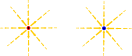
\includegraphics[scale=1]{images/sumidero-fuente.pdf}
\caption[Ley de Gauss]{Sumideros y fuentes respectivamente.}
\label{fig:2}
\end{figure}

La \textit{ley de Gauss magnética} nos dice que no existen monopolos magnéticos, los cuales serían los análogos magnéticos de las cargas. Dicho de otro modo, una superficie cerrada ubicada en cualquier punto del espacio siempre tendrá un flujo de campo magnético neto igual a 0. Esto puede entenderse al ver la figura \ref{fig:3} en donde se intenta esquematizar un dipolo magnético, y en particular, se puede observar que cada linea de campo siempre intercepta la superficie cerrada en dos ocasiones, una desde el polo positivo hacia fuera de la superficie (saliendo) y otra desde fuera de la superficie hasta el polo negativo (entrando), dando como resultado un flujo de campo magnético nulo.
\begin{figure}[!ht]
\centering
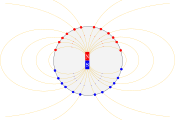
\includegraphics[scale=0.7]{images/ley-de-gauss-magnetismo.pdf}
\caption[Ley de Gauss para magnetismo]{Dipolo magnético dentro de superficie cerrada.}
\label{fig:3}
\end{figure}

La \textit{ley de Faraday} nos explica cómo funcionan los efectos de inducción magnética, esto quiere decir que si tengo un campo magnético variando en el tiempo, a su vez, éste inducirá un campo eléctrico.  Y la \textit{ley de Ampère-Maxwell} complementa lo anterior diciendo que un campo eléctrico variando en el tiempo inducirá un campo magnético. De esta forma podemos hacer notar que no solo las cargas e imanes son los culpables de influir en los campos eléctricos y magnéticos respectivamente, si no que también una fuente de campo magnético puede ser un campo eléctrico variando en el tiempo y viceversa.

Una de las importantes consecuencias de estas ecuaciones es que ellas implican la \textit{ley de conservación de la carga eléctrica} o \textit{ecuación de continuidad}. En particular, si calculamos la divergencia del rotor del campo magnético obtenemos que
\begin{align}
\div{\curl{\vb{B}}} &= \div{ \left( \pdv{\vb{E}}{t} + 4\pi \vb{J} \right) }\\
&= 4\pi \pdv{\rho}{t} + 4\pi \div{\vb{J}}\\
&= 0.
\end{align}

\section{Formulación covariante}

En el año 1905, el físico alemán Albert Einstein (1879-1955) presentó en su trabajo titulado \textit{Zur Elektrodynamik Bewegter Körper} \cite{Einstein} (``Sobre la electrodinámica de los cuerpos en movimiento'') presentó por primera vez su Teoría Especial de la Relatividad basada en dos postulados, los cuales eran
\begin{itemize}
\item[1)] las leyes de la Física son invariantes en todos los sistemas de referencia inerciales,
\item[2)] la velocidad de la luz en el vacío es igual para todos los observadores, independiente del movimiento de la fuente de luz.
\end{itemize}

Pese a las inconsistencias de su teoría con la mecánica Newtoniana, el trabajo de Einstein logró solucionar uno de los mayores problemas de la época, pero antes de explicarlo es necesario ponernos en contexto.

Como se presentó anteriormente, Maxwell logra unificar con sus ecuaciones toda la teoría electromagnética en 4  ecuaciones el año 1865, sin embargo dichas ecuaciones presentaban un problema y era que éstas no eran invariantes bajo transformaciones de Galileo. Esto quiere decir que, si consideramos un observador inercial $O$ y otro observador $O'$ moviéndose con velocidad constante $\vb{v}$ respecto a $O$, las ecuaciones de Maxwell respecto a $O'$ son diferentes y, por ende, implicaría la existencia de observadores privilegiados en el Universo lo cual va en contra del primer principio mostrado anteriormente. Bajo esta lógica las ecuaciones de Maxwell debieran ser erróneas, sin embargo en todos los experimentos en los cuales se les ponía a prueba, no lograban evidenciar inconsistencias entre las ecuaciones y los resultados experimentales, dando a entender que las predicciones hechas por dichas ecuaciones eran correctas. El problema era simple, las ecuaciones de Maxwell eran incorrectas o las transformaciones que se utilizaban para relacionar los observadores $O$ y $O'$ lo eran.

No fue hasta que Einstein presenta su teoría en donde muestra las transformaciones de Lorentz como medio para relacionar observadores inerciales, y cómo éstas mantienen la invariancia de las ecuaciones de Maxwell.

Al pasar los años, varios experimentos han logrado corroborar la teoría de Relatividad Especial (SR por sus siglas en inglés), explicando así efectos de los cuales antes no se conocía su existencia, como por ejemplo la dilatación temporal.

Por otro lado, y pese a que la teoría de SR permitía solucionar el problema de las ecuaciones de Maxwell, también era necesario asegurar que la teoría electromagnética fuera compatible con los principios que Einstein postuló en su teoría. Por esta razón se define el \textit{tensor de Faraday}
\begin{equation}
F^{\mu \nu} := \mqty*(
0 & -E^x & -E^y & -E^z \\
E^x & 0 & -B^z & B^y \\
E^y & B^z & 0 & -B^x \\
E^z & -B^y & B^x & 0 \\ 
),
\end{equation}
lo cual permite reescribir las ecuaciones inhomogéneas de Maxwell (la \textit{ley de Gauss} y la \textit{ley de Ampère-Maxwell}) de una forma más compacta como
\begin{equation}
\label{eq:1}
\partial_{\mu} F^{\mu \nu} = 4\pi J^{\nu},
\end{equation}
donde $J^{\mu} := \rho_0 u^{\mu}$ es la 4-densidad de corriente, $\rho_0$ es la densidad de carga respecto a un observador co-móvil con la fuente y $u^{\mu}$ es la 4-velocidad de las cargas.

También es posible reescribir las ecuaciones homogéneas de Maxwell como
\begin{equation}
\label{eq:2}
\partial_{[\mu} F_{\nu \lambda]} = 0.
\end{equation}

\subsection{Tensor dual}

Existe otra forma de escribir \eqref{eq:2} con el fin de que se parezca más a \eqref{eq:1}, dicha forma es introducir la definición del tensor dual. Sea $A^{\mu \nu}$ un tensor bajo transformaciones lineales de coordenadas, se define el dual como
\begin{equation}
\dual{A}^{\mu \nu} := \frac{1}{2} \epsilon^{\mu \nu \lambda \rho} A_{\lambda \rho},
\end{equation}
donde $\epsilon^{\mu \nu \lambda \rho}$ es el pseudo-tensor de Levi-civita definido en el Apéndice \ref{ape:convenciones}.

También notamos que es posible obtener la relación inversa, es decir, a partir del tensor dual obtener el tensor original
\begin{equation}
A^{\mu \nu} = -\frac{1}{2} \epsilon^{\mu \nu \lambda \rho} \dual{A}_{\lambda \rho}.
\end{equation}

A partir de lo anterior, el tensor electromagnético dual es
\begin{equation}
\label{eq:3}
\dual{F}^{\mu \nu} := \mqty*(
0 & -B^x & -B^y & -B^z \\
B^x & 0 & -E^z & E^y \\
B^y & E^z & 0 & -E^x \\
B^z & -E^y & E^x & 0 \\ 
),
\end{equation}
lo cual, en este caso, es equivalente a reemplazar $\vb{E}$ por $\vb{B}$ y viceversa.

Finalmente, de las ecuaciones homogéneas de Maxwell pueden ser escritas usando el tensor dual como
\begin{equation}
\partial_{\mu} \dual{F}^{\mu \nu} = 0.
\end{equation}

\section{Fuerzas de marea}
\label{sec:1}

En mecánica newtoniana, usamos el término \textbf{fuerzas de marea} para referirnos a los efectos de las inhomoeneidades del campo gravitacional (el cual produce diferentes aceleraciones en masas de prueba ubicadas en diferentes puntos del espacio). Por ejemplo si consideramos dos masas puntuales de prueba, en caída libre y separadas una distancia infinitesimal, un observador en caída libre junto con ellas apreciará que, mientras están cayendo, éstas se acercan entre sí, experimentando una aparente fuerza entre ellas.

Siguiendo el ejemplo anterior, sean $\vb{x}_1$ y $\vb{x}_2$ las posiciones de ambas masas de prueba, y tales que $\vb{x}_2 = \vb{x}_1 + \delta \vb{x}$, la aceleración con la que ambas masas caen son $g_i[\vb{x}_1]$ y $g_i[\vb{x}_2]$ respectivamente (ver figura \ref{fig:4}). 
\begin{figure}[h!]
\centering
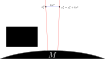
\includegraphics[scale=1.2]{images/desvio.pdf}
\caption[Esquema de desvío]{Esquema de los efectos de las inhomogeneidades del campo gravitacional.}
\label{fig:4}
\end{figure}

En particular, la aceleración de la segunda masa es
\begin{equation}
g_i[x+\delta x] = g_i[x] + \left( \partial_j g_i[x] \right) \delta x_j + \mathcal{O}(x^2).
\end{equation}

Podemos definir la aceleración relativa entre ambas masas como
\begin{equation}
\delta g_i = g_i[x+\delta x] - g_i[x] \approx \left( \partial_j g_i[x] \right) \delta x_j,
\end{equation}
y como la aceleración a su vez es definida como la segunda derivada temporal de la posición, la ecuación anterior puede ser escrita como
\begin{equation}
\label{eq:122}
\dv[2]{ }{t} \delta x_i = (\partial_j g_i) \delta x_j.
\end{equation}

Como podemos ver, todo esto nace del hecho que el campo gravitacional no es igual en todos los puntos del espacio, lo mismo ocurre con el campo electromagnético. Si consideramos dos cargas con el mismo cociente $q/m$ separadas infinitesimalmente, siendo afectadas por la presencia de un campo electromagnético externo , y describiendo un movimiento parametrizado por el mismo parámetro $\tau$. Entonces las fuerzas que afecta a ambas cargas son, respectivamente,
\begin{equation}
\label{eq:4}
\dv[2]{x_1^{\mu}}{\tau} = \frac{q}{m} F^{\mu}_{\ \nu}[x_1] \dv{x_1^{\nu}}{\tau}, \qquad 
\dv[2]{x_2^{\mu}}{\tau} = \frac{q}{m} F^{\mu}_{\ \nu}[x_2] \dv{x_2^{\nu}}{\tau},
\end{equation}
donde $x_1^{\mu}$ y $x_2^{\mu}$ son las curvas descritas por la primera y segunda carga respectivamente. Expandiendo el tensor de Faraday hasta primer orden en serie de Taylor, se obtiene que
\begin{equation}
F^{\mu}_{\ \nu}[x_2] = F^{\mu}_{\ \nu}[x_1 + \delta x] \approx F^{\mu}_{\ \nu}[x_1] + \partial_{\sigma} F^{\mu}_{\ \nu}[x_1] \delta x^{\sigma}.
\end{equation}

Así 
\begin{equation}
\label{eq:5}
\dv[2]{x_2^{\mu}}{\tau} = \dv[2]{ }{\tau} \left( x_1^{\mu} + \delta x^{\mu} \right) = \frac{q}{m} \left( F^{\mu}_{\ \nu}[x_1] + \partial_{\sigma} F^{\mu}_{\ \nu}[x_1] \delta x^{\sigma} \right) \dv{ }{\tau} \left( x_1^{\nu} + \delta x^{\nu} \right),
\end{equation}
y reemplazando \eqref{eq:5} en la definición $\delta x^{\mu} := x_2^{\mu} - x_1^{\mu}$, se obtiene que
\begin{equation}
\dv[2]{ }{\tau} \delta x^{\mu} = \frac{q}{m} \left[ F^{\mu}_{\ \nu} \dv{ }{\tau} \delta x^{\nu} + \partial_{\gamma} F^{\mu}_{\ \nu} u^{\nu} \delta x^{\gamma} + \partial_{\gamma} F^{\mu}_{\ \nu} \delta x^{\gamma} \dv{ }{\tau} \delta x^{\nu} \right].
\end{equation}

Por último, si se asume que
\begin{equation}
\left| \dv{\tau} \delta x^{\mu} \right| \ll |u^{\mu}|,
\end{equation}
es decir, la 4-velocidad de las cargas definida como $u^{\mu}_{1,2} := \mathrm{d}x^{\mu}_{1,2}/\mathrm{d}\tau $ son aproximadamente iguales, se tiene que
\begin{equation}
\label{eq:6}
\dv[2]{ }{\tau} \delta x^{\mu} = \frac{q}{m} \left( \partial_{\gamma} F^{\mu}_{\ \nu} \right) u^{\nu} \delta x^{\gamma},
\end{equation}
que representa las inhomogeneidades del campo electromagnético.

\section{Expansión multipolar}
\label{sec:2}

Si consideramos una distribución compacta de carga y corriente respectivamente, podemos hacer uso del método de expansión multipolar para calcular los valores del potencial escalar y vectorial en todos los puntos del espacio. Para esto es necesario describir todos los puntos de la distribución en cuestión respecto un punto de referencia $O$ (usualmente elegido en un punto al interior de ésta). Entonces para un punto lejano $\vb{x}$ (es decir, a una distancia mucho más grande que el tamaño de la distribución) escribimos los potenciales como una suma infinita de términos descritos en términos de $\vb{x}'$ (los cuales representan los puntos de la distribución respecto al punto $O$) y finalmente, bajo la hipótesis de que $|\vb{x}| \gg |\vb{x}'|$, introducimos la definición de los momentos multipolares para cada elemento de la expansión.
\begin{figure}[h!]
\centering
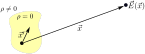
\includegraphics[scale=1]{images/multipolar.pdf}
\caption[Expansión multipolar electromagnética]{Expansión multipolar en electromagnetismo.}
\end{figure}

Por ejemplo, para una distribución electroestática de carga, sabemos que el potencial escalar de dicha carga viene dado por
\begin{equation}
\Phi(\vb{x}) = \int_{\Omega} \frac{\rho(\vb{x})}{|\vb{x} - \vb{x}'|} d^3x,
\end{equation}
donde $\Omega$ son los puntos que componen la distribución. Como podemos observar, es necesario resolver la integral la cual, en general, es complicado desde un punto de vista matemático. No obstante, haciendo uso de la expansión en serie de Taylor podemos notar que
\begin{align}
\frac{1}{|\vb{x} - \vb{x}'|} &= \frac{1}{|\vb{x}|} - x'_a \partial_a \left( \frac{1}{|\vb{x} - \vb{x}'|} \right)_{x'=0} + \frac{1}{2!} x'_a x'_b \partial_a \partial_b \left( \frac{1}{|\vb{x} - \vb{x}'|} \right)_{x'=0} + \dots,\\
&= \frac{1}{|\vb{x}|} - x'_a \partial_a \frac{1}{|\vb{x}|} + \frac{1}{2!} x'_a x'_b \partial_a \partial_b \frac{1}{|\vb{x}|} + \dots,\\
&= \frac{1}{r}  - x'_a \partial_a \frac{1}{r} + \frac{1}{2!} x'_a x'_b \partial_a \partial_b \frac{1}{r} + \dots,\\
&= \sum_{n=0}^{\infty} \frac{(-1)^n}{n!} x'_{a_1} \dots x'_{a_n} \partial_{a_1} \dots \partial_{a_n} \frac{1}{r},
\end{align}
y así
\begin{equation}
\Phi(\vb{x}) = \sum_{n=0}^{\infty} Q_{a_1 a_2 \dots a_n} \partial_{a_1} \partial_{a_2} \dots \partial_{a_n} \frac{1}{r},
\end{equation}
donde $Q_{i_1 i_2 \dots i_n}$ son los momentos multipolares eléctricos definidos como
\begin{equation}
Q_{a_1 a_2 \dots a_n} := \int_{\Omega} x_{a_1} x_{a_2} \dots x_{a_n} \rho(\vb{x}) d^3x.
\end{equation}

Usando la misma idea podemos definir los momentos multipolares magnéticos
\begin{equation}
M_{a_1 a_2 \dots a_n b} := \int_{\Omega} x_{a_1} x_{a_2} \dots x_{a_n} J_b(\vb{x}) \  d^3x,
\end{equation}
y así reescribir el potencial vectorial como
\begin{equation}
A_a(\vb{x}) = \sum_{n=0}^{\infty} \frac{(-1)^n}{n!} M_{a_1 a_2 \dots a_n b} \partial_{a_1} \partial_{a_2} \dots \partial_{a_n} \frac{1}{r}.
\end{equation}

Podemos entender lo anterior como dos expansiones multipolares diferentes, una para el caso eléctrico y otra para el caso magnético, sin embargo, es posible reformular dichas expansiones a fin de introducir el tensor de Faraday y con ello obtener una versión relativista para dicha expansión.

A partir de la fuerza de Lorentz podemos ver que
\begin{equation}
\label{eq:106}
F^{\mathrm{EM}}_{\mu} = \int_{\Omega} F_{\mu \nu}(x') J^{\nu}(x') \mathrm{d}V',
\end{equation}
y expandiendo en serie de Taylor el tensor de Faraday se obtiene que
\begin{equation}
\label{eq:107}
F_{\mu \nu}(x') = F_{\mu \nu}(X + \delta x) = F_{\mu \nu}(X) +  \partial_{\gamma} F_{\mu \nu}(X) \delta x^{\gamma} +  \frac{1}{2} \partial_{\xi} \partial_{\gamma} F_{\mu \nu}(X) \delta x^{\gamma} \delta x^{\xi} + \dots,
\end{equation}
donde $X$ denota la línea de mundo de $O$ y $\delta x$ la diferencia de coordenadas de una vecindad de puntos respecto de $O$. Así hasta primer orden, la ecuación \eqref{eq:106} se transforma en
\begin{equation}
\label{eq:121}
F^{\mathrm{EM}}_{\mu} = F_{\mu \nu}(X) \int_{\Omega} J^{\nu} \mathrm{d}V' + \partial_{\gamma} F_{\mu \nu}(X) \int_{\Omega} J^{\nu} \delta x^{\gamma} \mathrm{d}V'.
\end{equation}

Definiendo los momentos multipolares como
\begin{align}
\label{eq:108}
M^{\mu} &:= \int_{\Omega} J^{\mu} \mathrm{d}V',\\
\label{eq:109}
M^{\mu \nu} &:= \int_{\Omega} J^{\mu} \delta x^{\nu} \mathrm{d}V',\\
M^{\mu \nu \gamma} &:= \int_{\Omega} J^{\mu} \delta x^{\nu} \delta x^{\gamma} \mathrm{d}V',\\
\vdots & \qquad \vdots \nonumber \\
M^{\mu \nu \dots \gamma} &:= \int_{\Omega} J^{\mu} \delta x^{\nu} \dots \delta x^{\gamma} \mathrm{d}V',
\end{align}
se puede re-escribir \eqref{eq:121} como
\begin{equation}
F^{\mathrm{EM}}_{\mu} = F_{\mu \nu}(X) M^{\nu} + \partial_{\gamma} F_{\mu \nu}(X) M^{\nu \gamma}.
\end{equation}


\subsection{Dipolo magnético}

Se define un dipolo magnético como una distribución idealizada que solo posee momento dipolar no-nulo, es decir $M^{\mu \nu} \neq 0$, $M^{\mu} = 0$ y $M^{\mu \nu \dots \gamma} = 0$. Podemos calcular la fuerza que experimenta una distribución modelada hasta el orden dipolar en dicha expansión, producto de un campo magnético externo independiente del tiempo, es decir $\vb{E}=0$. Así, el campo magnético externo es descrito por el tensor de Faraday, mientras que los momentos multipolares describen el dipolo magnético, y la fuerza de Lorentz representa la fuerza que ejerce el campo magnético externo sobre el dipolo.

Al estar considerando $X^{\mu}$ como las coordenadas de la línea de mundo de referencia para describir los elementos de la distribución en cuestión, es necesario notar que al introducir la componente temporal en la formulación, es necesario fijar un tiempo en el cual se realiza esta descripción, dando a entender que para un instante de tiempo $t_0$, la componente $X^0$ siempre igual a las componentes $x^0$ de los puntos que conforman la vecindad de $O$ y así se deduce que $\delta x^0 = 0$, lo cual al introducir en \eqref{eq:109} se obtiene que $M^{\mu 0} = 0$, y al ser el campo externo puramente magnético, entonces $M^{(\mu \nu)} = 0$, teniendo así que solo las componentes con índices espaciales son no-nulas. Luego podemos definir el momento magnético $\mu$ implícitamente como
\begin{equation}
\label{eq:110}
M^{i j} = \epsilon^{i j k} \mu_k,
\end{equation}
y finalmente, introduciendo \eqref{eq:108}, \eqref{eq:109} y \eqref{eq:110} en \eqref{eq:107}, se obtiene que
\begin{equation}
F^{\mathrm{EM}}_{\mu} = \epsilon^{i j k} \mu_k \partial_i F_{\mu j},
\end{equation}
lo cual, para un observador co-móvil con el dipolo es
\begin{equation}
F^{\mathrm{EM}}_{\mu} = \epsilon^{\gamma \nu \sigma \rho} \partial_{\nu} F_{\mu \sigma} \mu_{\rho} u_{\gamma}.
\end{equation}

Si deseamos extender el análisis a fin de introducir momentos multipolares de orden superior en la expansión, es posible seguir un desarrollo similar, obteniendo que las ecuaciones de movimiento para una distribución modelada más momentos multipolares son
\begin{align}
\label{eq:111}
\dv{p_{\mu}}{s} &= -\sum_{n=1}^N \frac{n}{(n+1)!} m^{\nu_1 \nu_2 \dots \nu_n \lambda} \partial_{\mu} \partial_{(\nu_2} \dots \partial_{\nu_n} F_{\nu_1) \lambda},\\
\label{eq:112}
\dv{S^{\mu \nu}}{s} &= 2 p^{[\mu} u^{\nu]} + 2 \sum_{n=0}^{N-1} \frac{1}{n!} \eta^{\sigma [\kappa} m^{\lambda] \rho_1 \dots \rho_n \mu} \partial_{\rho_1} \partial_{\rho_2} \dots \partial_{\rho_n} F_{\sigma \mu},
\end{align}
donde $m^{\mu_1 \dots \mu_n}$ son los momentos multipolares definidos en \cite{Dixon1, Dixon2, Dixon3}, $u^{\mu} := \mathrm{d} X^{\mu} / \mathrm{d}s$ es la 4-velocidad de $O$, $p^{\mu}$ es el 4-momento de las cargas y $\eta^{\mu \nu}$ la métrica del espaciotiempo plano (ver Apéndice \ref{ape:convenciones}).						%Capitulo Electrodinamica covariante
\newpage
\chapter{Relatividad General}
\label{cap:2}
\newpage

\section{Gravedad}

Luego de sus contribuciones sobre el estudio de los cuerpos a velocidades relativistas y de establecer una nueva formulación para la teoría electromagnética clásica consistente con sus aportes en Relatividad Especial, se había generado a su vez un nuevo problema: ¿cómo introducir la interacción gravitacional en su nueva teoría?.

No fue si no hasta 10 años después, en 1915, cuando en su trabajo titulado \textit{Grundgedanken der allgemeinen Relativitätstheorie und Anwendung dieser Theorie in der Astronomie} \cite{Einstein-2} (``Idea básica de la teoría general de la relatividad y aplicación de esta teoría en astronomía''), Einstein plantea una nueva forma de entender la gravedad, dicha formulación se conoce como \textbf{la Teoría de la Relatividad General}. 

Esta teoría está basada principalmente en un principio (postulado por el mismo Einstein), el cual plantea que \textit{``El movimiento de un cuerpo producto de un campo gravitacional depende únicamente de su posición inicial en el espaciotiempo, no de su constitución. Y el resultado de cualquier experimento local, gravitacional o no, en un laboratorio en caída libre todos los efectos de la gravedad desaparece''}. Este principio recibe el nombre de \textbf{Principio de equivalencia fuerte} y plantea que, básicamente, no hay diferencia entre la gravedad provocada por los objetos con masa, y los efectos de los sistema de referencia no inerciales\footnote{\url{http://teoria-de-la-relatividad.blogspot.com/2009/03/8-el-principio-de-equivalencia.html}} como se muestra en la figura \ref{fig:5}. Cabe mencionar que existe otro principio muy similar llamado \textbf{Principio de equivalencia débil}, el cual fue planteado por Galileo y plantea que \textit{el movimiento de cualquier partícula de prueba en caída libre es independiente de su composición y estructura}. Comúnmente, este principio es utilizado para explicar el porqué los cuerpos en el vacío siempre caen con la misma aceleración, independiente de su masa.
\begin{figure}[!ht]
\centering
\begin{subfigure}{0.3\textwidth}
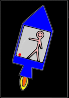
\includegraphics[width=\textwidth]{images/principio-equivalencia-1.pdf}
\caption{Cohete}
\end{subfigure}
\begin{subfigure}{0.3\textwidth}
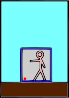
\includegraphics[width=\textwidth]{images/principio-equivalencia-2.pdf}
\caption{Tierra}
\end{subfigure}
\caption[Principio de equivalencia de Einstein]{Esquema explicativo del principio de equivalencia propuesto por Einstein.}
\label{fig:5}
\end{figure}

Una de las primeras predicciones de dicha teoría fue el cálculo del ángulo de deflexión de un haz de luz al pasar una distancia $R$ de un cuerpo central, efecto que fue verificado en 1919 a mano de Arthur Eddingon \textit{et.al.} \footnote{\url{https://es.wikipedia.org/wiki/Arthur_Stanley_Eddington/media/Archivo:1919_eclipse_positive.jpg}} \cite{Coles} (ver \ref{fig:6}), siendo éste uno de los primeros grandes avances sobre esta nueva forma de entender la gravedad.
\begin{figure}[!ht]
\centering
\includegraphics[scale=0.5]{images/1919eclipse.jpg}
\caption[Fotografía tomada por Eddintong]{Fotografía original tomada por Eddintong en 1919.}
\label{fig:6}
\end{figure}

\section{Ecuaciones de campo}
\label{sec:3}

Una de las razones principales de porqué Einstein tardó tanto en completar su teoría fue la necesidad de estudiar los avances en \textbf{Geometría diferencial}, área de las Matemáticas que se dedica al estudio de la geometría utilizando diversas herramientas del cálculo y álgebra. Los principales objetos de estudio en esta disciplina son las variedades diferenciales las cuales, principalmente, representan un espacio topológico que localmente se reduce al espacio Euclidiano.

Siendo más específico, Einstein se centró en el estudio de la geometría riemanniana para desarrollar su teoría, el cual tiene como elemento principal la \textbf{métrica}. Dicho elemento matemático nos permite definir el concepto de distancia y es representado por una matriz simétrica de $4 \cross 4$ con elementos reales.

Volviendo al contexto físico, Einstein logra asociar dicho elemento matemático a una propiedad intrínseca del espaciotiempo y muestra cómo la métrica es determinada por los elementos que conforman el espacio (energía), y el cómo la métrica a su vez determina la trayectoria de los objetos que se mueven en dicho espaciotiempo, dando origen a la famosa frase \textit{La materia le dice al espacio cómo curvarse, y el espacio le dice a la materia cómo moverse}\footnote{\url{https://es.wikiquote.org/wiki/John_Archibald_Wheeler}}.

Esta relación viene determinada por un conjunto de 10 ecuaciones diferenciales parciales no-lineales llamadas las ecuaciones de campo de Einstein,
\begin{equation}
\label{eq:7}
R_{\mu \nu} - \frac{1}{2}R g_{\mu \nu} = 8\pi  T_{\mu \nu},
\end{equation}
donde $R_{\mu \nu}$ es el tensor de Ricci, $R$ el escalar de curvatura, $g_{\mu \nu}$ la métrica del espaciotiempo, $T_{\mu \nu}$ el tensor de energía-momentum, $G$ la constante de gravitación universal y $c$ la velocidad de la luz en el vacío (ver Apéndice \ref{ape:convenciones}).

\subsection{Solución de Kerr}

La primera solución exacta de \eqref{eq:7} fue encontrada el año 1916 por el físico alemán Karl Schwarzschild (1873-1916) \cite{Heinicke}, dicha solución muestra cómo es la métrica al rededor de una distribución de masa $M$ esféricamente simétrica no-rotante, muchos nuevos conceptos son introducidos con esta nueva solución, como lo son el radio de Schwarzschild y el horizonte de eventos.

No fue hasta 1963 cuando el físico neozelandés Roy Kerr (1934-ahora) \cite{Heinicke} logra encontrar una nueva solución exacta a \eqref{eq:7}, la cual muestra cómo es la métrica fuera agujero negro rotante de masa $M$ y momento angular $J$, la cual es (en coordenadas de Boyer-Lindquist y expresada en términos de su elemento de línea)
\begin{equation}
\label{eq:8}
\mathrm{d}s^2 = \frac{\Delta}{\rho^2} \left( \mathrm{d}t - a \sin^2 \theta \mathrm{d}\phi \right)^2 - \frac{\sin^2 \theta}{\rho^2} \left[ (r^2 + a^2)\mathrm{d}\phi - a\mathrm{d}t \right]^2 - \frac{\rho^2}{\Delta} \mathrm{d}r^2 - \rho^2 \mathrm{d}\theta^2,
\end{equation}
donde: 
\begin{equation}
\rho^2 := r^2 + a^2 \cos^2 \theta ,\quad \Delta := r^2 - 2r + a^2, \quad m := GM, \quad a := \frac{J}{M}.
\end{equation}

Las principales propiedades de esta métrica son que es estacionaria y axialmente simétrica, de lo cual se puede inferir que hay dos vectores de Killing los cuales son $\partial_t$ y $\partial_{\phi}$, y por último, que la métrica es invariante bajo la transformación
\begin{eqnarray*}
t &\longrightarrow & -t ,\\
\phi &\longrightarrow & -\phi,
\end{eqnarray*} 

\section{Ecuación de desvío geodésico}

Como se muestra en la sección \ref{sec:1}, el estudio de las inhomogeneidades del campo gravitacional newtoniano y el campo electromagnético determinan las fuerzas de marea. En el contexto de Relatividad General es posible estudiar el mismo problema.

Consideremos $g_{\mu \nu}$ como la métrica del espaciotiempo, y consideremos una trayectoria parametrizada por $x^{\mu}(s)$. Se define la derivada covariante de $A^{\mu}$ sobre la curva como
\begin{equation}
\label{eq:9}
\cd{A^{\mu}} := \dv{A^{\mu}}{s} + \Gamma^{\mu}_{\rho \sigma} \dv{x^{\rho}}{\s} A^{\sigma},
\end{equation}
donde $s$ es un parámetro afín, $\Gamma^{\mu}_{\rho \sigma}$ son los símbolos de Christoffel de segunda especie (ver Apéndice \ref{ape:convenciones}). 

Se puede ver que si $x^{\mu}(s)$ es una geodésica, entonces
\begin{equation}
\cd{ } \left[ \dv{x^{\mu}}{\s} \right] = 0.
\end{equation} 

\begin{lemma}
\label{lema:1}
Sean $G_1$ y $G_2$ dos geodésicas parametrizadas por el mismo parámetro afín $s$ y separadas una distancia infinitesimal, si $x^{\mu}_1(s)$ y $x^{\mu}_2(s)$ son las parametrizaciones de ambas geodésicas respectivamente, y se define la 4-velocidad como $u^{\mu}(s) := \mathrm{d}x^{\mu}_1/\mathrm{ds}$, entonces la segunda derivada covariante sobre la curva $x^{\mu}_1$ de $\delta x^{\mu}:= x^{\mu}_2 - x^{\mu}_1$ es
\begin{equation}
\label{eq:10}
\frac{\delta^2}{\mathrm{ds}^2}\delta x^{\mu} = \dv[2]{\delta x^{\mu}}{\s} + \partial_{\nu} \Gamma^{\mu}_{\rho \sigma} u^{\rho} u^{\sigma} \delta x^{\nu} - R^{\mu}_{\ \rho \sigma \nu} u^{\rho} u^{\nu} \delta x^{\sigma} + 2 \Gamma^{\mu}_{\sigma \rho} u^{\sigma} \dv{ }{\s} \delta x^{\rho}, 
\end{equation}
donde $R^{\mu}_{\ \rho \sigma \nu}$ es el tensor de Riemann.
\end{lemma}
\begin{proof}

De \eqref{eq:9} sabemos que
\begin{align}
\frac{\delta^2}{\mathrm{ds}^2}\delta x^{\mu} &= \cd{ } \left[ \cd{ } \delta x^{\mu} \right] \nonumber \\
&= \dv{ }{\s} \left[ \cd{ } \delta x^{\mu} \right] + \Gamma^{\mu}_{\rho \sigma} u^{\rho} \cd{ } \delta x^{\sigma} \nonumber \\
\label{eq:81}
&= \dv[2]{ }{\s} \delta x^{\mu} + \dv{ }{\s} \left[ \Gamma^{\mu}_{\rho \sigma} u^{\rho} \delta x^{\sigma} \right] + \Gamma^{\mu}_{\rho \sigma} u^{\rho} \dv{ }{\s}\delta x^{\sigma} + \Gamma^{\mu}_{\rho \sigma} \Gamma^{\sigma}_{\alpha \beta} u^{\rho} u^{\alpha} \delta x^{\beta}.
\end{align}

El segundo término en \eqref{eq:81} puede ser escrito como
\begin{equation}
\label{eq:11}
\dv{ }{\s} \left[ \Gamma^{\mu}_{\rho \sigma} u^{\rho} \delta x^{\sigma} \right]
=
\left( \dv{ }{\s} \Gamma^{\mu}_{\rho \sigma} \right) u^{\rho} \delta x^{\sigma} + \Gamma^{\mu}_{\rho \sigma} \left(  \dv{ }{\s} u^{\rho} \right) \delta x^{\sigma} + \Gamma^{\mu}_{\rho \sigma} u^{\rho} \left( \dv{ }{\s} \delta x^{\sigma} \right).
\end{equation}

Además, por la regla de la cadena sabemos que
\begin{equation}
\label{eq:12}
\dv{ }{\mathrm{s}} \Gamma^{\mu}_{\rho \sigma} = \partial_{\lambda} \Gamma^{\mu}_{\rho \sigma} u^{\lambda},
\end{equation}
y, como $x_1^{\mu}(s)$ es una geodésica,
\begin{equation}
\label{eq:13}
\dv{u^{\mu}}{\mathrm{s}} + \Gamma^{\mu}_{\rho \sigma} u^{\rho} u^{\sigma} = 0.
\end{equation}

Reemplazando \eqref{eq:12} y \eqref{eq:13} en \eqref{eq:11},
\begin{equation}
\label{eq:14}
\dv{ }{\s} \left[ \Gamma^{\mu}_{\rho \sigma} u^{\rho} \delta x^{\sigma} \right]
=
\partial_{\lambda} \Gamma^{\mu}_{\rho \sigma} u^{\rho} \delta x^{\sigma} - \Gamma^{\mu}_{\rho \sigma} \Gamma^{\rho}_{\alpha \beta} u^{\alpha} u^{\beta} \delta x^{\sigma} + \Gamma^{\mu}_{\rho \sigma} u^{\rho} \dv{ }{\s} \delta x^{\sigma}.
\end{equation}

Luego, \eqref{eq:14} en \eqref{eq:81},
\begin{equation}
\label{eq:15}
\frac{\delta^2}{\mathrm{ds}^2}\delta x^{\mu} = \dv[2]{ }{\mathrm{s}} \delta x^{\mu} + 
\left[ \partial_{\sigma} \Gamma^{\mu}_{\rho \nu} + \Gamma^{\mu}_{\delta \sigma} \Gamma^{\delta}_{\rho \nu} - \Gamma^{\mu}_{\delta \nu} \Gamma^{\delta}_{\rho \sigma}  \right] u^{\rho} u^{\sigma} \delta x^{\nu} + 2\Gamma^{\mu}_{\alpha \beta} u^{\alpha} \dv{ }{\mathrm{s}} \delta x^{\nu}.
\end{equation}

Por la definición del tensor de Riemann \ref{ape:convenciones} se puede ver que
\begin{equation}
\label{eq:16}
R^{\mu}_{\ \nu \rho \sigma} + \partial_{\sigma} \Gamma^{\mu}_{\rho \rho} = \partial_{\rho} \Gamma^{\mu}_{\rho \sigma} + \Gamma^{\mu}_{\rho \delta} \Gamma^{\delta}_{\nu \sigma} - \Gamma^{\mu}_{\sigma \delta} \Gamma^{\delta}_{\nu \rho},
\end{equation}
así
\begin{equation}
\frac{\delta^2}{\mathrm{ds}^2}\delta x^{\mu} = \dv[2]{\delta x^{\mu}}{\s} + \left( \partial_{\nu} \Gamma^{\mu}_{\rho \sigma} \right) u^{\rho} u^{\sigma} \delta x^{\nu} - R^{\mu}_{\ \rho \sigma \nu} u^{\rho} u^{\nu} \delta x^{\sigma} + 2 \Gamma^{\mu}_{\sigma \rho} u^{\sigma} \dv{ }{\s} \delta x^{\rho},
\end{equation}
lo cual prueba el lemma.
\end{proof}

\begin{theorem}
\label{teo:1}
Sean $G_1$ y $G_2$ dos geodésicas parametrizadas por el mismo parámetro afín $s$, separadas infinitesimalmente, y si 
$$|\dv{ }{\s} \delta x^{\rho}| \ll |u^{\rho}(s)|$$
es decir, los vectores tangentes a las geodésicas definidos como $u^{\mu}_{1,2}(s) := \mathrm{d}x^{\mu}_{1,2}/\mathrm{ds}$ son aproximadamente iguales. Entonces la segunda derivada covariante a lo largo de $x^{\mu}_1$ de $\delta x^{\mu}$ es
\begin{equation}
\label{eq:17}
\frac{\delta^2}{\mathrm{ds}^2}\delta x^{\mu} = - R^{\mu}_{\ \sigma \nu \rho} u^{\sigma} u^{\nu} \delta x^{\rho}.
\end{equation}
\end{theorem}
\begin{proof}
Para dos geodésicas se sabe que
\begin{equation}
\cd{ }\left[ \dv{x_1^{\mu}}{\mathrm{s}} \right] = \cd{ }\left[ \dv{x_2^{\mu}}{\mathrm{s}} \right] = 0,
\end{equation}
luego
\begin{equation}
\label{eq:18}
\dv[2]{x_1^{\mu}}{\mathrm{s}} + \Gamma^{\mu}_{\rho \sigma} \dv{x^{\rho}}{\mathrm{s}} \dv{x^{\sigma}}{\mathrm{s}} = 0,
\end{equation}
donde los símbolos de Christoffel están evaluados a lo largo de $x_1$. Para la segunda geodésica sabemos que $x_2^{\mu} = x_1^{\mu} + \delta x^{\mu}$, así
\begin{equation}
\label{eq:19}
\dv[2]{x_1^{\mu}}{\mathrm{s}} + \dv[2]{ }{\mathrm{s}} \delta x^{\mu} + \Gamma^{\mu}_{\rho \sigma} \dv{ }{\mathrm{s}} \left( x_1^{\rho} + \delta x^{\rho} \right) \dv{ }{\mathrm{s}} \left( x_1^{\sigma} + \delta x^{\sigma} \right) = 0,
\end{equation}
donde en este caso, los símbolos de Christoffel están evaluados a lo largo de $x_2=x_1 + \delta x$. 

Expandiendo hasta primer orden se obtiene que
\begin{equation}
\label{eq:20}
\Gamma^{\mu}_{\rho \sigma}[x + \delta x] = \Gamma^{\mu}_{\rho \sigma}[x] + \partial_{\nu} \Gamma^{\mu}_{\rho \sigma}[x] \delta x^{\nu} + \mathcal{O}(\delta x^2).
\end{equation}

Reemplazando \eqref{eq:20} en \eqref{eq:19}, encontramos que hasta primer orden en $\delta x$,
\begin{equation}
0 = \dv[2]{x_1^{\mu}}{\mathrm{s}} + \dv[2]{ }{\mathrm{s}} \delta x^{\mu} + \left( \Gamma^{\mu}_{\rho \sigma}[x] + \left( \partial_{\nu} \Gamma^{\mu}_{\rho \sigma}[x] \right) \delta x^{\nu} \right) \dv{ }{\mathrm{s}} \left( x_1^{\rho} + \delta x^{\rho} \right) \dv{ }{\mathrm{s}} \left( x_1^{\sigma} + \delta x^{\sigma} \right).
\end{equation}

Luego, definiendo $u^{\mu} := \mathrm{d} x^{\mu}_1 / \mathrm{ds}$,
\begin{equation}
\label{eq:21}
0 = \dv[2]{x_1^{\mu}}{\mathrm{s}} + \dv[2]{ }{\mathrm{s}} \delta x^{\mu} + \Gamma^{\mu}_{\rho \sigma} u^{\rho} u^{\sigma} + \left( \partial_{\lambda} \Gamma^{\mu}_{\rho \sigma} \right) u^{\rho} u^{\sigma} \delta x^{\lambda} + 2 \Gamma^{\mu}_{\rho \sigma} u^{\rho} \dv{ }{\mathrm{s}} \delta x^{\sigma}. 
\end{equation}

Así, reemplazando \eqref{eq:18} en \eqref{eq:21} se deduce que
\begin{equation}
0 = \dv[2]{ }{\mathrm{s}} \delta x^{\mu} + \partial_{\lambda} \Gamma^{\mu}_{\rho \sigma} u^{\rho} u^{\sigma} \delta x^{\lambda} + 2 \Gamma^{\mu}_{\rho \sigma} u^{\rho} \dv{ }{\mathrm{s}} \delta x^{\sigma}.
\end{equation}

Finalmente, usando el lema \ref{lema:1} encontramos que
\begin{equation}
\frac{\delta^2}{\mathrm{ds}^2}\delta x^{\mu} = - R^{\mu}_{\ \sigma \nu \rho} u^{\sigma} u^{\nu} \delta x^{\rho},
\end{equation}
lo cual prueba el teorema.
\end{proof}

La ecuación \eqref{eq:17} describe las inhomogeidades de la curvatura y es conocida como la \textbf{ecuación de desvío geodésico}.

\section{Campos gravitacionales débiles}

Como se dijo en la sección \ref{sec:3}, las ecuaciones de campo de Einstein son no-lineales en la métrica, y por ende, sus soluciones no dependen linealmente del tensor energía-momentum. Además, como dicho tensor, el cual se encuentra en el lado derecho de \eqref{eq:7} está multiplicado por $G$, entonces las soluciones dependerán no-linealmente de $G$.

Es bien sabido que la solución de ecuaciones no-lineales es un área de las matemáticas de difícil estudio, puesto que al no ser lineales, no existen métodos generales para poder resolverlas. Es por esto que se han desarrollado métodos aproximados para resolver dichas ecuaciones, en particular, es posible utilizar un método perturbativo para determinar las soluciones de \eqref{eq:7} como una serie infinita de términos.

Si usamos coordenadas pseudo-euclidianas y consideramos pequeñas perturbaciones de la forma
\begin{equation}
g_{\mu \nu} = \eta_{\mu \nu} + h_{\mu \nu}, \qquad |h_{\mu \nu}| \leq 1,
\end{equation}
donde $\eta_{\mu \nu} = \mathrm{diag}(1,-1,-1,-1)$ corresponde a la métrica plana, y si separamos las perturbaciones en una serie de órdenes en potencias de G, se puede escribir que
\begin{equation}
\label{eq:120}
g_{\mu \nu} = \eta_{\mu \nu} + h_{\mu \nu}^{(1)} + h_{\mu \nu}^{(2)} + \dots.
\end{equation}

Además de hacer la expansión de la métrica en distintos órdenes en $h$, es posible realizar una expansión similar para cada cantidad relevante en geometría riemanniana, así
\begin{align}
\label{eq:116}
\Gamma^{\lambda}_{\mu \nu} &= \Gamma^{(1)\lambda}_{\mu \nu} + \Gamma^{(2)\lambda}_{\mu \nu} + \dots,\\
\label{eq:117}
R_{\mu \nu} &= R_{\mu \nu}^{(1)} + R_{\mu \nu}^{(1)} + \dots,\\
\label{eq:118}
G_{\mu \nu} &= G_{\mu \nu}^{(1)} + G_{\mu \nu}^{(2)} + \dots,\\
\label{eq:119}
T_{\mu \nu} &= T_{\mu \nu}^{(0)} + T_{\mu \nu}^{(1)} + \dots.
\end{align}

El primer término de los símbolos de Christoffel en \eqref{eq:116}, el tensor de Ricci en \eqref{eq:117} y el tensor de Einstein en \eqref{eq:118} son cero, puesto que al ser proporcionales a derivadas de la métrica, y como el primer orden en \eqref{eq:120} es constante, entonces estas cantidades comienzan del orden 1.

De esta forma, las ecuaciones de campo de Einstein se pueden escribir como
\begin{equation}
G_{\mu \nu}^{(1)} + G_{\mu \nu}^{(2)} + \dots = \frac{8 \pi G}{c^4} \left( T_{\mu \nu}^{(0)} + T_{\mu \nu}^{(1)} + \dots \right),
\end{equation}
que puede ser separada en distintos órdenes como
\begin{align}
G_{\mu \nu}^{(1)} &= \frac{8 \pi G}{c^4} T_{\mu \nu}^{(0)},\\
G_{\mu \nu}^{(2)} &= \frac{8 \pi G}{c^4} T_{\mu \nu}^{(1)},\\
G_{\mu \nu}^{(3)} &= \frac{8 \pi G}{c^4} T_{\mu \nu}^{(2)},\\
\nonumber
& \vdots
\end{align}

Note que siempre se asocia cada orden del tensor de Einstein, a un orden menor del tensor de energía-momentum. Esto es por que la expansión es en términos de $G$, y al haber un $G$ multiplicando a $T_{\mu \nu}$, entonces la combinación $GT_{\mu \nu}^{(0)}$ es de orden 1.

\subsection{Expansión a primer orden}
\subsubsection{Métrica inversa}

A primer orden en $G$ se tiene que la métrica del espaciotiempo adpota la forma de
\begin{equation}
g_{\mu \nu} = \eta_{\mu \nu} + h_{\mu \nu}^{(1)},
\end{equation}
por convención, se suben y bajan los índices usando la métrica plana.

La primera cantidad necesaria a obtener es la métrica inversa, usando la propiedad que $\delta^{\mu}_{\nu} = g^{\mu \lambda} g_{\nu \lambda}$, y que
\begin{equation}
g^{\mu \nu} = \eta^{\mu \nu} + g^{\mu \nu}_{(1)} + \mathcal{O}(G^2),
\end{equation}
se obtiene que 
\begin{equation}
g^{\mu \nu}_{(1)} = -h^{\mu \nu}_{(1)} := -\eta^{\mu \lambda} \eta^{\nu \rho} h_{\lambda \rho}^{(1)}.
\end{equation}

\subsubsection{Conexión}
A primer orden, el primer término en la serie de los símbolos de Christoffel es:
\begin{equation}
\Gamma^{(1)\lambda}_{\mu \nu} = \frac{1}{2} \left( \partial_{\mu} h^{\lambda}_{(1) \nu} + \partial_{\nu} h^{\lambda}_{(1) \mu} - \partial^{\lambda} h_{\mu \nu}^{(1)} \right).
\end{equation}

\subsubsection{Tensor de Riemann}
Por otra parte, el primer orden del tensor de curvatura es:
\begin{equation}
\label{eq:85}
R^{\rho}_{(1) \mu \nu \lambda} = \frac{1}{2} \left( \partial_{\mu} \partial_{\nu} h^{\rho}_{(1) \lambda} - \partial_{\mu} \partial_{\lambda} h^{\rho}_{(1) \nu} + \partial_{\lambda} \partial^{\rho} h_{\mu \nu}^{(1)} - \partial_{\nu} \partial^{\rho} h_{\mu \lambda}^{(1)} \right).
\end{equation}

A partir del tensor de Riemann, es posible contraer índices para obtener todas las demás cantidades subsecuentes, tales como el tensor de Ricci, el escalar de curvatura y el tensor de Einstein.

\section{Expansión multipolar en GR}

En Física los problemas siempre involucran cuerpos extendidos (con volumen), lo cual en muchos casos representa un gran problema matemático a la hora de trabajar ecuaciones. Por esta razón se definen cantidades como el centro de masa, punto al que se le asignan propiedades del sistema completo (como masa o velocidad). Si bien esta forma de trabajar simplifica el análisis, al ser solo una aproximación, algunos efectos no pueden ser descritos usando solo el centro de masa \cite{nataly}.

Algo similar ocurre en Relatividad General: si se desea estudiar el comportamiento de un cuerpo extendido sería necesario considerar un \textit{tubo de mundo} en vez de una \textit{línea de mundo} como usualmente se hace con partículas puntuales.

La idea a grandes rasgos es reemplazar el tubo de mundo $\Sigma$ por una línea de mundo $L$, y el tensor de energía-momentum $T^{\mu \nu}$ por un conjunto de momentos multipolares $t^{\mu \nu}, t^{\mu \nu \sigma}, t^{\mu \nu \sigma \lambda}, \cdots$ a lo largo de $L$ (ver figura \ref{fig:1}), y donde la ley de balance del tensor energía-momentum permite determinar la evolución de dichos momentos multipolares.
\begin{figure}[!ht]
	\centering
	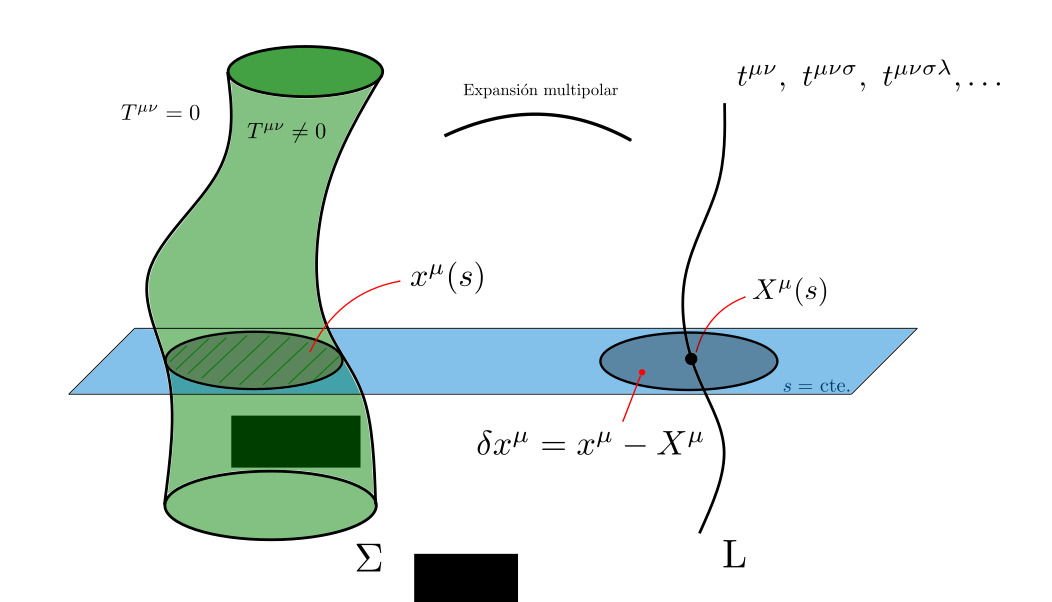
\includegraphics[scale=0.45]{images/papapetrou.pdf}
	\caption[Expansión multipolar en RG]{Esquema de la abstracción de tubo de mundo a línea de mundo}
	\label{fig:1}
\end{figure}
En el año 1951, el físico griego-francés Achille Papapetrou (1907-1997) en su trabajo titulado ``\textit{Spinning test-particles in general relativity. I}"" \cite{Papapetrou2,Papapetrou1} deriva por primera vez un método para obtener las ecuaciones de movimiento para cuerpos que poseen estructura interna, lo cual permitía introducir nuevas propiedades a dichos cuerpos como por ejemplo rotación interna (spin). 

Con el pasar de los años, se han desarrollado métodos alternativos para obtener las mismas ecuaciones sin los problemas que presentaban originalmente las ecuaciones de Papapetrou, entre los cuales destaca el carácter no-covariante de las ecuaciones de movimiento, esto por separar en el cálculo las componentes temporales y espaciales.

En \cite{Steinhoff-Puetzfeld} se utiliza la ecuación de conservación covariante del tensor de energía momentum
\begin{equation}
\label{eq:22}
\nabla_{\nu} T^{\mu \nu} = 0,
\end{equation}
de forma que se pueda escribir el tensor energía-momentum como la expansión en una serie de momentos multipolares, para luego obtener una conjunto de condiciones a satisfacer por los coeficientes de la expansión. De esta forma
\begin{align}
\nonumber
\tilde{T}^{\mu \nu} &= \int^{+\infty}_{-\infty} \left[ t^{\mu \nu} \delta_{(4)}(x^{\mu} - X^{\mu}(s)) + \nabla_{\lambda} [t^{\lambda \mu \nu} \delta_{(4)}(x^{\mu} - X^{\mu}(s))] \right.\\
&\quad \left.  + \nabla_{\rho} \nabla_{\lambda} [t^{\rho \lambda \mu \nu} \delta_{(4)}(x^{\mu} - X^{\mu}(s))] +  \dots
\right] \mathrm{d}s,
\end{align}
corresponde a la expansión de $\tilde{T}$, donde $t^{\mu \nu \dots}$ son los momentos multipolares, $\delta_{(4)}$ es la delta de Dirac 4-dimensional, $X^{\mu}(s)$ la parametrización de la curva de referencia que representa el tubo de mundo, y $s$ el parámetro afín con el cual se describe la curva. También es necesario mencionar que la cantidad que se escribe en términos de los momentos multipolares es la densidad tensorial de energía-momentum (ver Apéndice \ref{ape:convenciones}), esto es por la presencia de la delta de Dirac en su expansión.

También es necesario definir lo que en \cite{Tulczyjew} es llamada como \textit{forma canónica}. Se dice que una densidad tensorial arbitraria $\tilde{A}^{c_1 c_2 \dots}$ se encuentra en su forma canónica si puede ser escrita de la forma
\begin{equation}
\tilde{A}^{c_1 c_2 \dots} = \sum_{k=0}^{m} \int_{-\infty}^{+\infty} \nabla_{c_1 c_2 \dots c_k} \left[ \alpha^{c_1 \dots c_k b_1 \dots b_n} \delta_{(4)}(x^{\mu} - X^{\mu}(s)) \right], 
\end{equation}
donde los coeficientes satisfacen que
\begin{align}
\alpha^{c_1 \dots c_k b_1 \dots b_n} &= \alpha^{(c_1 \dots c_k) b_1 \dots b_n},\\
u_{c_1}\alpha^{c_1 \dots c_k b_1 \dots b_n} &= 0,
\end{align}
y se define el vector tangente a lo largo de la trayectoria como $u^{\mu} := \mathrm{d}X^{\mu} / \mathrm{d}s$.

\begin{theorem}
\label{teo:2}
Si para una densidad tensorial escrita en su forma canónica $\tilde{A}^{b_1 \dots b_n}$ y un arbitrario campo tensorial $T_{b_1 \dots b_n}$ se tiene que
\begin{equation}
\int_{\Omega}  \tilde{A}^{b_1 \dots b_n}T_{b_1 \dots b_n} = 0,
\end{equation}
en una región arbitraria del espaciotiempo $\Omega$, entonces todos los coeficientes de la expansión $\alpha^{c_1 \dots c_k b_1 \dots b_n}$ son nulos.
\end{theorem}

La demostración de este teorema puede encontrarse en \cite{Tulczyjew}.

\subsection{Descomposiciones respecto la velocidad}

Consideraremos que de forma general, los momentos multipolares satisfacen las siguientes simetrías:
\begin{equation}
t^{\lambda_1 \dots \lambda_n \mu \nu} = t^{\lambda_1 \dots \lambda_n (\mu \nu)}, \qquad t^{\lambda_1 \dots \lambda_n \mu \nu} = t^{(\lambda_1 \dots \lambda_n) \mu \nu}.
\end{equation}

Con ayuda del proyector $\rho^{\mu}_{\ \nu} := \delta^{\mu}_{\ \nu} - u^{\mu}u_{\nu}$, podemos hacer una descomposición de cada momento multipolar en términos de sus componentes ortogonales a $u^{\mu}$, recordando que $u^{\mu}u_{\mu} = 1$. Así, para el momento monopolar se tiene que
\begin{equation}
\label{eq:23}
t^{\mu \nu} = \ \des{0}{o}^{\mu \nu} + 2 \des{0}{o}^{(\mu} u^{\nu )} + \des{0}{t} u^{\mu} u^{\nu},
\end{equation}
donde
\begin{align*}
\des{0}{o}^{\mu \nu} &:=  \rho^{\mu}_{\ \lambda} \rho^{\nu}_{\ \sigma} t^{\lambda \sigma},\\
\des{0}{o}^{\mu} &:= \rho^{\mu}_{\ \lambda} u_{\nu} t^{\lambda \nu},\\
\des{0}{t} &:= t^{\mu \nu} u_{\mu} u_{\nu}.
\end{align*}

Para el momento dipolar se tiene que
\begin{equation}
\label{eq:24}
t^{\mu \nu \gamma} = \ \des{1}{o}^{\mu \nu \gamma} + 2 \des{1}{o}^{\mu ( \nu} u^{\gamma )} + \des{1}{o}^{\mu} u^{\nu} u^{\gamma} + u^{\mu} t^{\nu \gamma},
\end{equation}
donde
\begin{align*}
\des{1}{o}^{\mu \nu \gamma} &:= \rho^{\mu}_{\ \sigma} \rho^{\nu}_{\ \rho} \rho^{\gamma}_{\ \lambda} t^{\sigma \rho \lambda},\\
\des{1}{o}^{\mu \nu} &:= \rho^{\mu}_{\ \sigma} \rho^{\nu}_{\ \rho} u_{\lambda} t^{\sigma \rho \lambda},\\
\des{1}{o}^{\mu} &:= \rho^{\mu}_{\ \sigma} u_{\rho} u_{\lambda} t^{\sigma \rho \lambda},\\
\des{1}{t}^{\mu \nu} &:= t^{\lambda \mu \nu} u_{\lambda}.
\end{align*}

Y para el momento cuadrupolar se tiene que
\begin{equation}
\des{2}{t}^{\mu \nu \gamma \delta} = \ \des{2}{o}^{\mu \nu \gamma \delta} + 2 \des{2}{o}^{\mu \nu (\gamma} u^{\delta)} + \des{2}{o}^{\mu \nu} u^{\gamma} u^{\delta} - u^{\mu} u^{\nu} \des{2}{t}^{\gamma \delta} + 2 u^{(\mu} \des{2}{t}^{\nu) \gamma \delta},
\end{equation}
donde
\begin{align*}
\des{2}{o}^{\mu \nu \gamma \delta} &:= \rho^{\mu}_{\ \sigma} \rho^{\nu}_{\ \rho} \rho^{\gamma}_{\ \lambda} \rho^{\delta}_{\ \xi} t^{\sigma \rho \lambda \xi},\\
\des{2}{o}^{\mu \nu \gamma} &:= \rho^{\mu}_{\ \sigma} \rho^{\nu}_{\ \rho} \rho^{\gamma}_{\ \lambda} u_{\xi} t^{\sigma \rho \lambda \xi},\\
\des{2}{o}^{\mu \nu} &:= \rho^{\mu}_{\ \sigma} \rho^{\nu}_{\ \rho} u_{\lambda} u_{\xi} t^{\sigma \rho \lambda \xi},\\
\des{2}{t}^{\mu \nu \gamma} &:= t^{\mu \nu \gamma \xi} u_{\xi},\\
 \des{2}{t}^{\mu \nu} &:= t^{\mu \nu \gamma \xi} u_{\gamma} u_{\xi}.
\end{align*}

Luego, se obtendrán distintas condiciones a satisfacer para cada elemento de la descomposición derivando así las ecuaciones de movimiento.

\subsection{Partícula monopolo}

Si hacemos una expansión hasta el primer orden en la expansión multipolar, es decir, escribimos la densidad tensorial de energía-momentum como
\begin{equation}
\tilde{T}^{\mu \nu} = \int_{-\infty}^{+\infty} \mathrm{d}s t^{\mu \nu} \delta_{(4)},
\end{equation}
donde la integral es sobre la curva, respecto a $\mathrm{d}s$ en el intervalo $(-\infty,+\infty)$, y la delta de Dirac está evaluada en $x^{\mu} - X^{\mu}(s)$.

A partir de \eqref{eq:22} se obtiene que
\begin{equation}
\label{eq:25}
\int_{-\infty}^{+\infty} \mathrm{d}s \nabla_{\mu} [ t^{\mu \nu} \delta_{(4)}] = 0.
\end{equation}

Por otro lado, utilizando el proyector podemos notar que
\begin{equation}
\rho^{\mu}_{\ \gamma} t^{\gamma \nu} = t^{\mu \nu} - u^{\mu} u_{\gamma} t^{\gamma nu}
\quad \Longleftrightarrow \quad t^{\mu \nu} = \rho^{\mu}_{\ \gamma} t^{\gamma \nu} + u^{\mu} u_{\gamma} t^{\gamma nu},
\end{equation}
definiendo la notación $t^{\mu \hat{\nu} \gamma} := \rho^{\nu}_{\sigma} t^{\mu \sigma \gamma} $, entonces  \eqref{eq:25} se puede reescribir como
\begin{equation}
\label{eq:26}
\int_{-\infty}^{+\infty} \mathrm{d}s \nabla_{\nu} [(t^{\hat{\nu} \mu} + u^{\nu} u_{\sigma} t^{\sigma \mu} )] = 0.
\end{equation}

Es posible demostrar que (ver apéndice \ref{ape:1}) la integral satisface
\begin{equation}
\label{eq:88}
\int_{-\infty}^{+\infty} \mathrm{d}s \nabla_{\nu} [u^{\nu} T^{\mu_1 \mu_2 \dots} \delta_{(4)}] = \int_{-\infty}^{+\infty} \mathrm{d}s \cd{T^{\mu_1 \mu_2 \dots}} \delta_{(4)}.
\end{equation}

De esta forma la ecuación \eqref{eq:26} implica que
\begin{equation}
\label{eq:27}
\int_{-\infty}^{+\infty} \mathrm{d}s \cd{} [u_{\nu} t^{\nu \mu}] \delta_{(4)} + \int_{-\infty}^{+\infty} \mathrm{d}s \nabla_{\nu} [t^{\hat{\nu} \mu} \delta_{(4)}] = 0,
\end{equation}
aplicando el teorema se deduce que
\begin{align}
\cd{} [u_{\nu} t^{\nu \mu}] &= 0,\\
t^{\hat{\nu} \mu} &= 0.
\end{align}

Utilizando la descomposición \eqref{eq:23}, se obtienen las siguientes condiciones para los elementos de la descomposición
\begin{align}
\label{eq:28}
\cd{} [\des{0}{o}^{\mu} + u^{\mu} \des{0}{t}] &= 0,\\
\label{eq:29}
\des{0}{o}^{\mu \nu} + \des{0}{o}^{\mu} u^{\nu} &= 0.
\end{align}

Contrayendo \eqref{eq:29} con respecto a la 4-velocidad se puede inferir que
\begin{equation}
\label{eq:30}
\des{0}{o}^{\mu \nu} = 0 \quad \mathrm{y \ que} \quad \des{0}{o}^{\mu} = 0.
\end{equation}

A partir de \eqref{eq:28} y \eqref{eq:30} se puede observar que
\begin{equation}
\des{0}{t} = \mathrm{cte.} \quad \mathrm{y} \quad \cd{u^{\mu}} = 0.
\end{equation}

Así, hasta primer orden, las ecuaciones de movimiento para la partícula se reducen a la ecuación de la geodésica.

\subsection{Partícula monopolo-dipolo}

Si extendemos el análisis hasta segundo orden en la expansión multipolar, entonces la ecuación \eqref{eq:22} implica que
\begin{equation}
\label{eq:31}
\int_{-\infty}^{+\infty} \mathrm{d}s \nabla_{\mu} [ t^{\mu \nu} \delta_{(4)}] + \int_{-\infty}^{+\infty} \mathrm{d}s \nabla_{\gamma}\nabla_{\mu} [ t^{\mu \gamma \nu} \delta_{(4)}] = 0,
\end{equation}
antes de utilizar el teorema \ref{teo:2} es necesario escribir \eqref{eq:31} en su forma canónica.

Es conveniente notar antes que:
\begin{equation}
\label{eq:32}
\nabla_{[\mu} \nabla_{\nu]} T^{\mu \nu \gamma} \equiv \frac{1}{2} R_{\mu \nu \sigma}^{\ \ \ \ \gamma} T^{\mu \nu \sigma}.
\end{equation}

Por otro lado, el segundo término en \eqref{eq:31} puede ser reescrito, usando el proyector como
\begin{align}
\nonumber
\int_{-\infty}^{+\infty} \mathrm{d}s \nabla_{\mu} \nabla_{\sigma} [ t^{\sigma \mu \nu} \delta_{(4)} ] &= 
\int_{-\infty}^{+\infty} \mathrm{d}s \nabla_{\mu} \nabla_{\sigma} [ ( t^{\hat{\sigma} \hat{\mu} \nu} + t^{\hat{\sigma} \rho \nu} u^{\mu} u_{\rho} + t^{\rho \hat{\mu} \nu} u^{\sigma} u_{\rho} + u^{\sigma} u^{\mu} u_{\rho} u_{\delta} t^{\rho \delta \nu} ) \delta_{(4)} ] \\ \nonumber
&= \int_{-\infty}^{+\infty} \mathrm{d}s \delta_{(4)} \frac{\delta^2}{\mathrm{d}s^2} t^{\mu \rho \nu} u_{\mu} u_{\rho} + \int_{-\infty}^{+\infty} \mathrm{d}s \nabla_{\nu} \left[ \cd{} (t^{\rho \hat{\mu} \nu} u_{\rho}) \delta_{(4)} + \cd{u^{\mu}} u_{\rho} u_{\gamma}  t^{\rho \gamma \nu} \delta_{(4)} \right] \\ 
\label{eq:33}
& \quad + \int_{-\infty}^{+\infty} \mathrm{d}s \nabla_{\mu} \nabla_{\gamma} \left[ ( t^{\hat{\gamma} \hat{\mu} \nu}  + t^{\hat{\gamma} \rho \nu} u^{\mu} u_{\rho}) \delta_{(4)} \right].
\end{align}

Utilizando \eqref{eq:32} vemos que
\begin{equation}
\label{eq:34}
\int_{-\infty}^{+\infty} \mathrm{d}s \nabla_{\mu} \nabla_{\gamma} \left[ (t^{\hat{\gamma} \rho \nu} u^{\mu} u_{\rho}) \delta_{(4)} \right] = \int_{-\infty}^{+\infty} \mathrm{d}s \nabla_{\gamma} \left[ \delta_{(4)} \cd{} t^{\hat{\gamma} \rho \nu} \right] + \int_{-\infty}^{+\infty} \mathrm{d}s R^{\ \ \ \ \nu}_{\mu \gamma \delta} u^{\mu} u_{\rho} t^{\hat{\gamma} \rho \delta}.
\end{equation}

Reemplazando \eqref{eq:27}, \eqref{eq:33} y \eqref{eq:34} en \eqref{eq:31} es posible obtener que
\begin{align}
\nonumber
0 &= \int_{-\infty}^{+\infty} \mathrm{d}s \left[ \frac{\delta^2}{\mathrm{d}s^2} (t^{\gamma \rho \nu} u_{\gamma}u_{\rho}) + \cd{} (t^{\gamma \nu} u_{\gamma}) + \frac{1}{2} R^{\ \ \ \ \nu}_{\mu \gamma \delta} (2 u^{\mu} u_{\rho} t^{\hat{\gamma} \rho \delta} + t^{\hat{\gamma} \hat{\mu} \delta}) \right] \delta_{(4)} + \int_{-\infty}^{+\infty} \mathrm{d}s \nabla_{\mu} \nabla_{\gamma} \left[ ( t^{\hat{\gamma} \hat{\mu} \nu} )\delta_{(4)} \right] \\ 
\label{eq:35}
& \quad + \int_{-\infty}^{+\infty} \mathrm{d}s \nabla_{\mu} \left\{ \left[ \cd{} (t^{\rho \hat{\mu} \nu} u_{\rho} + t^{\hat{\mu} \rho \nu} u_{\rho}) + \cd{u^{\mu}} u_{\rho} u_{\delta} t^{\rho \delta \nu} + t^{\hat{\mu} \nu} \right] \delta_{(4)} \right\}.
\end{align}

De los primeros dos términos en la segunda línea en \eqref{eq:35} podemos ver que
\begin{align}
\nonumber
\frac{1}{2} \int_{-\infty}^{+\infty} \mathrm{d}s \nabla_{\mu} \left\{ \left[ \cd{}( t^{\rho \hat{\mu} \nu} u_{\rho} + t^{\hat{\mu} \rho \nu} u_{\rho}) \right] \right\} &= 
\int_{-\infty}^{+\infty} \mathrm{d}s \nabla_{\mu} \left\{ \left[ \rho^{\mu}_{\ \gamma} \cd{}( t^{(\gamma \rho) \nu} u_{\rho} ) - \cd{u^{\mu}} u_{\gamma} u_{\rho} t^{(\gamma \rho) \nu} \right] \delta_{(4)} \right\} \\ 
\label{eq:36}
& \quad - \int_{-\infty}^{+\infty} \mathrm{d}s \cd{} \left( \cd{u_{\gamma}} u_{\rho} t^{(\gamma \rho) \nu} \right) \delta_{(4)}.
\end{align}

Finalmente, si insertamos \eqref{eq:36} en \eqref{eq:35}, podemos obtener la forma canónica de \eqref{eq:31}:
\begin{align}
\nonumber
0 &= \int_{-\infty}^{+\infty} \mathrm{d}s \left[ \frac{\delta^2}{\mathrm{d}s^2} (t^{\gamma \rho \nu} u_{\gamma}u_{\rho}) + \cd{} (t^{\gamma \nu} u_{\gamma} - 2\cd{u_{\gamma}} u_{\rho} t^{(\gamma \rho) \nu}) + \frac{1}{2} R^{\ \ \ \ \nu}_{\mu \gamma \delta} (2 u^{\mu} u_{\rho} t^{\hat{\gamma} \rho \delta} + t^{\hat{\gamma} \hat{\mu} \delta}) \right] \delta_{(4)} \\ 
\label{eq:37}
& \quad + \int_{-\infty}^{+\infty} \mathrm{d}s \nabla_{\mu} \nabla_{\gamma} \left[ ( t^{\hat{\gamma} \hat{\mu} \nu} )\delta_{(4)} \right] + \int_{-\infty}^{+\infty} \mathrm{d}s \nabla_{\mu} \left\{ \left[ 2 \rho^{\mu}_{\ \gamma} \cd{}( t^{(\gamma \rho) \nu} u_{\rho} ) - \cd{u^{\mu}} u_{\gamma} u_{\rho} t^{\gamma \rho \nu} + t^{\hat{\mu} \nu} \right] \delta_{(4)} \right\}.
\end{align}

Aplicando el teorema \ref{teo:2}, del orden más alto en \eqref{eq:37} podemos ver que
\begin{equation}
0 =  t^{\hat{\gamma} \hat{\mu} \nu}.
\end{equation}

Usando \eqref{eq:24} se pueden obtener las siguientes dos condiciones para los elementos de la descomposición del momento dipolar,
\begin{equation}
\label{eq:38}
\des{1}{0}^{(\mu \nu)} = \ 0 \quad \mathrm{y \ que} \quad \des{1}{0}^{(\mu \nu) \gamma} = 0.
\end{equation}

Utilizando la identidad
\begin{equation}
\des{1}{0}^{\mu \nu \gamma} = \ \des{1}{0}^{(\mu \nu) \gamma} + \des{1}{0}^{(\gamma \mu) \nu} - \des{1}{0}^{(\nu \gamma) \mu},
\end{equation}
se deduce que
\begin{equation}
\label{eq:39}
\des{1}{0}^{\mu \nu \gamma} = 0.
\end{equation}

Del segundo orden en \eqref{eq:37} se obtiene que
\begin{equation}
2 \rho^{\mu}_{\ \gamma} \cd{}( t^{(\gamma \rho) \nu} u_{\rho} ) - \cd{u^{\mu}} u_{\gamma} u_{\rho} t^{\gamma \rho \nu} + t^{\hat{\mu} \nu} = 0,
\end{equation}
que al usar \eqref{eq:23} y \eqref{eq:24} nos lleva a
\begin{equation}
\rho^{\mu}_{\ \gamma} \cd{} ( \des{1}{o}^{\gamma \nu} + \des{1}{o}^{\gamma} u^{\nu} + \des{1}{t}^{\gamma \nu} )  + \des{0}{o}^{\mu \nu}  + \des{0}{o}^{\mu} u^{\nu} = 0,
\end{equation}
de donde al multiplicar con $u_{\nu}$ y $\rho^{\gamma}_{\ \nu}$ se obtienen dos condiciones para los elementos de la descomposición del momento monopolar
\begin{align}
\label{eq:40}
\des{0}{o}^{\mu} &= -u_{\rho} \rho^{\mu}_{\ \gamma} \cd{} (\des{1}{o}^{\gamma \rho} + \des{1}{o}^{\gamma} u^{\rho} + \des{0}{t}^{\gamma \rho}), \\
\label{eq:41}
\des{0}{o}^{\mu \nu} &= - \rho^{\mu}_{\ \gamma} \rho^{\nu}_{\rho} \cd{} (\des{1}{o}^{\gamma \rho} + \des{1}{o}^{\gamma} u^{\rho} + \des{0}{t}^{\gamma \rho}).
\end{align}

Tomando la parte antisimétrica de \eqref{eq:41} se obtiene que
\begin{equation}
\rho^{\mu}_{\ \gamma} \rho^{\nu}_{\ \rho} \cd{} (\des{1}{o}^{[\gamma \rho]} + \des{1}{o}^{[\gamma} u^{\rho]}) = 0,
\end{equation}
y al definir el tensor de espín como
\begin{equation}
\label{eq:42}
\des{1}{S}^{\mu \nu} := -2 (\des{1}{o}^{[\mu \nu]} + \des{1}{o}^{[\mu} u^{\nu]}),
\end{equation}
se deducen las ecuaciones de Papapetrou para la evolución del espín
\begin{equation}
\label{eq:83}
\cd{\des{1}{S}^{\mu \nu}} - u^{\mu} u_{\gamma} \cd{\des{1}{S}^{\gamma \nu}} - u^{\nu} u_{\gamma} \cd{\des{1}{S}^{\mu \gamma}} = 0.
\end{equation}

Por último, a partir del orden más bajo, a través del teorema \ref{teo:2}, \eqref{eq:23} y \eqref{eq:24} se obtiene que (ver Apéndice \ref{ape:3})
\begin{align}
\label{eq:43}
0 &= \cd{} \left( u_{\gamma} \cd{} \des{1}{t}^{\gamma \nu} + \des{0}{o}^{\nu} + \des{0}{t} u^{\nu} - \cd{u_{\gamma}} \des{1}{o}^{\gamma \nu} - \cd{\gamma} \des{1}{o}^{\gamma}u^{\nu} \right) \nonumber \\
& \quad + \frac{1}{2} R^{\ \ \ \ \nu}_{\mu \gamma \rho} \left[ 2u^{\mu}(\des{1}{o}^{\gamma \rho} + \des{1}{o}^{\gamma} u^{\rho}) + \des{1}{o}^{\gamma \mu \rho} + \des{1}{o}^{\gamma \mu}  u^{\rho}  \right],
\end{align}
donde al considerar \eqref{eq:39}, \eqref{eq:38} y \eqref{eq:42} se puede obtener que, a partir de \eqref{eq:43} las ecuaciones de Papapetrou para la evolución del 4-momentum (ver Apéndice \ref{ape:2})
\begin{equation}
\label{eq:82}
\cd{\des{1}{p}^{\mu}} = -\frac{1}{2} R^{\ \ \ \ \mu}_{\nu \gamma \rho} \des{1}{S}^{\nu \gamma} u^{\rho},
\end{equation}
donde se ha definido la masa y el 4-momentum como
\begin{align}
\des{1}{m} &:=\ \des{0}{t} - u_{\gamma} \cd{u_{\rho}} \des{1}{S}^{\gamma \rho} + u_{\gamma} u_{\rho} \cd{\des{1}{t}^{\gamma \rho}},\\
\label{eq:44}
\des{1}{p}^{\mu} &:=\ \des{1}{m} u^{\mu} + u_{\gamma} \cd{} \des{1}{S}^{\mu \gamma}.
\end{align}

De esta forma, las ecuaciones \eqref{eq:82} y \eqref{eq:83} determinan (en principio) la trayectoria de un objeto con estructura interna en un espaciotiempo arbitrario.

\subsubsection{Condiciones suplementarias y cantidades conservadas}

Como dijimos anteriormente, la idea de esta formulación es abstraer el tubo de mundo original (que describe las evolución de un cuerpo de forma completa) a una línea de mundo, la cual describe la evolución de un punto de referencia que se encuentra dentro del cuerpo extendido, pero que posee las propiedades del cuerpo original codificada en cada momento multipolar. Bajo esta idea, es necesario la elección de un punto de referencia antes de realizar la obtención de las ecuaciones de movimiento, ecuaciones que justamente describirán la evolución de dicho punto. Es por esta razón que las ecuaciones \eqref{eq:82} y \eqref{eq:83}, producto de la arbitrariedad en la elección de la curva de referencia, no describen completamente la evolución de los momentos multipolares. Así, para poder obtener una solución es necesario agregar lo que se le conoce como \textbf{condición suplementaria}.

En la literatura existen varias condiciones suplementarias de las cuales destacan dos que son,
\begin{center}
\begin{tabular}{cc}
\hline
Mathisson-Pirani & Tulcyjew \\
\hline \hline
$\des{1}{S}^{\mu \nu} u_{\nu} = 0 $ & $\des{1}{S}^{\mu \nu} \des{1}{p}_{\nu} = 0 $ \\
\hline
\end{tabular}
\end{center}

Podemos entender la utilidad de dichas condiciones suplementarias al hacer el siguiente análisis. La evolución de las cantidades definidas anteriormente pueden ser escritas de la siguiente forma (ver Apéndice \ref{ape:6}):
\begin{align}
\label{eq:45}
\cd{\des{1}{m}} &= \cd{u^{\mu}} \cd{}(u_{\nu} \des{1}{S}^{\mu \nu}),\\
\label{eq:103}
\cd{\des{1}{S}^{\mu \nu}} &= 2 \des{1}{p}^{[\mu} u^{\nu]},\\
\label{eq:46}
\cd{\des{1}{m'}} &:= \cd{}\sqrt{\des{1}{p}_{\mu}\des{1}{p}^{\mu}},\\
\label{eq:47}
\cd{\des{1}{S}^2} &:= \frac{1}{2} \cd{} \left( \des{1}{S}^{\mu \nu} \des{1}{S}_{\mu \nu} \right).
\end{align}

Como podemos observar, si consideramos la condición de Mathisson-Pirani las cantidades en \eqref{eq:45} y \eqref{eq:47} se conservan sobre la curva de referencia, mientras que si consideramos la condición de Tulcyjew las cantidades en \eqref{eq:46} y \eqref{eq:47} se conservan sobre la curva. Esto es importante puesto que mantener la conservación en cantidades como la masa del cuerpo en cuestión, o la magnitud del espín permiten determinar de forma consistente las soluciones a las ecuaciones de movimiento.

\subsection{Partícula monopolo-dipolo-cuadrupolo}

Si se extiende el desarrollo hasta el orden cuadrupolar, entonces la ecuación \eqref{eq:22} se pueden escribir como:
\begin{equation}
\label{eq:48}
\nabla_{\mu} \tilde{T}^{\mu \nu} = \int_{-\infty}^{+\infty} \mathrm{d}s \nabla_{\mu} [ t^{\mu \nu} \delta_{(4)}] + \int_{-\infty}^{+\infty} \mathrm{d}s \nabla_{\gamma}\nabla_{\mu} [ t^{\mu \gamma \nu} \delta_{(4)}] + \int_{-\infty}^{+\infty} \mathrm{d}s \nabla_{\rho} \nabla_{\gamma} \nabla_{\mu} [ t^{\gamma \mu \rho \nu} \delta_{(4)}] = 0.
\end{equation}

Luego de realizar desarrollo similar a los anteriores para obtener la forma canónica de \eqref{eq:48}, y de definir cantidades auxiliares como
\begin{align}
\des{0}{n} &:= \ \des{0}{t} + u_{\gamma} u_{\sigma} \left[ \cd{\des{1}{t}^{\gamma \sigma}} - \frac{\delta^2 \des{2}{t}^{\gamma \sigma}}{\mathrm{d}s^2} +2 \cd{} \left( u_{\delta} \cd{\des{2}{t}^{\delta \gamma \sigma}} + 2 u^{\delta} \des{2}{t}^{\mu \nu (\gamma} R_{\delta \mu \nu}^{\ \ \ \ \sigma)} \right) \right],\\
\des{1}{n}^{\mu} &:= \ \des{1}{o}^{\mu} + \rho^{\mu}_{\ \delta} u_{\gamma} u_{\sigma} \left( -\cd{u^{\delta} \des{2}{t}^{\gamma \sigma}} + 2\cd{\des{2}{t}^{\delta \gamma \sigma}} \right),\\
\des{1}{n}^{\mu \nu} &:= \ \des{1}{o}^{\mu \nu} + \rho^{\mu}_{\ \delta} \rho^{\nu}_{\ \gamma} u_{\sigma} \left( -\cd{u^{\delta} \des{2}{t}^{\gamma \sigma}} + 2\cd{\des{2}{t}^{\delta \gamma \sigma}} \right),\\
\des{2}{n}^{\mu \nu} &:= \ \des{2}{o}^{\mu \nu},\\
\des{2}{n}^{\mu \nu \gamma} &:= \ \des{2}{o}^{\mu \nu \gamma},\\
\des{2}{n}^{\mu \nu \gamma \delta} &:= \ \des{2}{o}^{\mu \nu \gamma \delta},
\end{align}
las ecuaciones de movimiento extendidas hasta el orden cuadrupolar son \cite{Steinhoff-Puetzfeld}
\begin{align}
\cd{\des{2}{S}^{\mu \nu}} &= 2\des{2}{p}^{[\mu} u^{\nu]} + \frac{4}{3} R_{\gamma \rho \sigma}^{\ \ \ \ [\mu} I^{\nu] \gamma \rho \sigma},\\
\label{eq:49}
\cd{\des{2}{p}^{\mu}} &= \frac{1}{2} R^{\mu}_{\ \ \nu \gamma \delta} u^{\nu} \des{2}{S}^{\gamma \delta} - g^{\mu \xi} \frac{1}{6} \nabla_{\xi} R_{\gamma \rho \delta \omega} I^{\gamma \omega \delta \rho},
\end{align}
donde los términos adicionales corresponden a las contribuciones de los momentos cuadrupolares y se definen como
\begin{align}
I^{\mu \nu \gamma \sigma} &:= 2\left( \des{2}{n}^{\mu \nu \gamma \sigma} + 2 \des{2}{n}^{\mu \nu (\gamma} u^{\sigma)} + 2\des{2}{n}^{\gamma \sigma (\mu} u^{\nu)} + 2\des{2}{n}^{\mu \nu} u^{\gamma} u^{\sigma} + 2\des{2}{n}^{\gamma \sigma} u^{\mu} u^{\nu} - 2 u^{(\mu} \des{2}{n}^{\nu)(\gamma} u^{\sigma)} \right),\\
\des{2}{S}^{\mu \nu} &:= -2 \left[ \des{1}{n}^{[\mu \nu]} + \des{1}{n}^{[\mu} u^{\nu]} - 2\left( \des{2}{n}^{\gamma [\mu \nu]} + \des{2}{n}^{\gamma [\mu} u^{\nu]} \right) \cd{u_{\gamma}} \right],\\
\des{2}{m} &:= \ \des{0}{n} + u_{\nu} \cd{u_{\mu}} \des{2}{S}^{\mu \nu} - \frac{2}{3} R_{\mu \nu \gamma}^{\ \ \ \ \sigma} \des{2}{n}^{\gamma \nu \mu} u_{\sigma},\\
\des{2}{p}^{\mu} &:= \ \des{2}{m} u^{\mu} + u_{\nu} \cd{\des{2}{S}^{\mu \nu}} + R_{\nu \gamma \sigma}^{\ \ \ \ \delta} \left( \frac{4}{3}\des{2}{n}^{\nu \mu \gamma \sigma} u_{\delta} + 4\des{2}{n}^{\mu \nu \sigma} u^{\gamma} u_{\delta} + \frac{4}{3} \des{2}{n}^{\nu \sigma \gamma} \rho^{\mu}_{\ \delta} + 2 \des{2}{n}^{\nu \sigma} u^{\gamma} \rho^{\mu}_{\ \delta} \right).
\end{align}

Cabe mencionar que el estudio de las cantidades \eqref{eq:45}, \eqref{eq:46} y \eqref{eq:47} puede ser extendido al orden cuadrupolar, determinando así que éstas no se conservan bajo las mismas condiciones suplementarias, lo cual podría dar pie a inferir que pueden existir cantidades suplementarias adicionales tales que estas cantidades sí se logren conservar bajo la curva. En \cite{Steinhoff-Puetzfeld-2} se logra encontrar una cantidad auxiliar que puede ser interpretada como la masa y se conserva hasta orden cuadrupolar. 			            %Cap�tulo Relatividad General
\newpage
\chapter{Analogía entre Relatividad General y la Teoría Electrodinámica Clásica}
\label{cap:3}
\newpage

\section{¿Porqué es importante el estudio de analogías en Física?}
\label{sec:4}
%SE PRESENTA UNA PEQUEÑA SECCIÓN DONDE SE MUESTRAN EJEMPLOS CONCRETOS DONDE EL ESTUDIO DE ANALOGÍAS EN FÍSICA HAN SERVIDO PARA DESAROLLAR/ENTENDER NUEVAS TEORÍAS


Antes de comenzar a hablar de analogías, debemos definir cómo entendemos una analogía en Física. Usualmente, usamos la palabra analogía cuando establecemos una relación entre dos cosas diferentes que en principio no tienen una conexión. Por ejemplo, la pintura es al pincel, lo que la música a los instrumentos\footnote{\url{https://www.ejemplos.co/20-ejemplos-de-analogias/ixzz5rKGc08QO}}.

De la misma forma, en el contexto físico podemos hacer algo similar si logramos construir una relación entre dos teorías diferentes como, por ejemplo, entre la teoría de la Relatividad General y la teoría de la Electrodinámica Clásica. Sin embargo, esa no es la única analogía existente.


En mecánica, los sistemas físicos que no poseen elementos con rotación (es decir, puramente traslacionales) pueden ser descritos completamente por medio de cantidades ya definidas como la masa $m$, fuerza $\vb{F}$, momentum lineal $\vb{p}$, posición $\vb{x}$, velocidad $\vb{v}$ y aceleración $\vb{a}$. No obstante, si estamos interesados en considerar los efectos de rotación en esos sistemas es útil introducir cantidades adicionales para poder describirlos, tales como el momento de inercia $I$, torque $\vb{\tau}$, el momentum angular $\vb{L}$, la posición angular $\theta$, la velocidad angular $\vb{\omega}$ y la aceleración angular $\vb{\alpha}$.

Como podemos notar (y si bien es cierto que las definiciones de dichas cantidades son diferentes) la interpretación a cada una de ellas es muy similar, de tal forma que podemos establecer una relación entre ellas a partir de su significado, como muestra la siguiente tabla.
\begin{center}
\begin{tabular}{c|c|l}
\hline
Caso traslacional & Caso rotacional & Magnitud\\
\hline \hline
$m$ & $I$ & Efectos de inercia \\
\hline
$\vb{p}$ & $\vb{L}$  & Cantidad de movimiento y rotación \\
\hline
$\vb{F}$ & $\vb{\tau}$ & Agentes externos actuando sobre el sistema \\
\hline
$\vb{x}$ & $\theta$ & Posición \\
\hline
$\vb{v}$ & $\vb{\omega}$ & Velocidad \\
\hline
$\vb{a}$ & $\vb{\alpha}$ & Aceleración\\
\hline
\end{tabular}
\end{center}

Y así, para cada cantidad en el caso traslacional hay una cantidad asociada en el caso rotacional. Pero ésa no es la única relación entre los elementos que describen los sistemas físicos en los casos traslacionales y rotantes, incluso las ecuaciones que describen esos sistemas son similares. Para los elementos en el caso traslacional, la ecuación principal para describirlos es la segunda ley de Newton
\begin{equation}
\sum_i \vb{F}_i = \dv{\vb{p}}{t},
\end{equation}
la cual nos dice que una variación temporal de la cantidad de movimiento es producto de los agentes externos que actúan en nuestro sistema. 

Y para sistemas rotantes, la ecuación principal para describirlos es
\begin{equation}
\sum_i \vb{\tau}_i = \dv{\vb{L}}{t},
\end{equation}
y equivalentemente al caso de movimiento traslacional, una variación temporal de la cantidad de rotación es igual al valor resultante de los agentes externos que actúan en nuestro sistema.

Muy a menudo, el estudio de sistemas que solo involucran elementos traslacionales es más fácil de entender que cuando se intentan estudiar sistemas con rotación, es por esto que la utilidad de esta analogía entre sistemas traslacionales y rotacionales nos puede permitir comprender sistemas más complejos. 

Este es el ejemplo más simple sobre el porqué una analogía puede ayudarnos a entender problemas más complicados en física.

\section{Tensores de marea}
Como se ha mencionado en las secciones anteriores, los elementos denominados fuerzas de marea son usados para describir los efectos de las inhomogeneidades de los campos. Podemos definir los tensores de marea para describir dichas fuerzas, por ejemplo en el caso newtoniano si definimos
\begin{equation}
K_{ij} (x) := - \partial_j g_i(x),
\end{equation}
las fuerzas de marea \eqref{eq:122} pueden ser escritas como
\begin{equation}
\dv[2]{ }{t}\delta x_i = -K_{ij}\delta x_j,
\end{equation}
donde $K_{ij}$ es el tensor de marea asociado.

En la teoría electromagnética y Relatividad General se puede hacer una definición similar, definidos los \textit{tensores de marea eléctricos y gravito-eléctricos} respectivamente como
\begin{equation}
\label{eq:50}
\mathtt{E}_{\mu \nu} := \left( \partial_{\nu} F_{\mu \gamma} \right) u^{\gamma}, \quad 
\mathrm{y } \quad \mathbb{E}_{\mu \nu} := R_{\mu \rho \nu \sigma} u^{\rho} u^{\sigma}.
\end{equation}
lo cual permite reescribir \eqref{eq:6} y \eqref{eq:17} de la siguiente forma:
\begin{equation}
\label{eq:130}
\dv[2]{ }{\s} \delta x_{\mu} = \frac{q}{m} \mathtt{E}_{\mu \nu} \ \delta x^{\nu}
,\qquad
\frac{\delta^2}{\mathrm{ds}^2} \delta x_{\mu} = - \mathbb{E}_{\mu \nu} \ \delta x^{\nu}.
\end{equation}

También se pueden definir sus contrapartes magnéticas como
\begin{equation}
\label{eq:51}
\mathtt{B}_{\mu \nu} := -\frac{1}{2} \epsilon_{\gamma \lambda \mu \alpha} \left( \partial_{\nu} F^{\gamma \lambda} \right) u^{\alpha}
,\quad \mathrm{y} \quad
\mathbb{H}_{\mu \nu} := -\frac{1}{2} \epsilon_{\gamma \lambda \mu \alpha} R^{\gamma \lambda}_{\ \ \nu \sigma} u^{\alpha} u^{\sigma},
\end{equation}
a las cuales nos referiremos como \textit{tensor de marea magnético} y \textit{tensor de marea gravito-magnético}.

La analogía propuesta en \cite{Costa-Herdeiro} pretende discutir cómo los efectos de las fuerzas de marea en los contextos gravitacionales y electromagéticos pueden ser comparados usando los tensores de marea.

Por otro lado, a partir de las definiciones de los tensores de marea podemos notar que es necesario conocer las derivadas del tensor de Faraday y el tensor de Riemann para construirlos. No obstante, también es posible obtener dichas cantidades si conocemos con anterioridad los tensores de marea, es decir, obtener una transformación inversa (ver Apéndice \ref{ape:4}). Ésta es
\begin{align}
\label{eq:52}
\partial_{\gamma} F_{\mu \nu} &= \epsilon_{\mu \nu \rho \sigma} \mathit{B}^{\rho}_{\ \gamma} u^{\sigma} - 2u_{[\mu} \mathit{E}_{\nu] \gamma},\\
\label{eq:53}
R_{\mu \nu \gamma \xi} u^{\xi} &= \epsilon_{\mu \nu \rho \sigma} \mathbb{H}^{\rho}_{\ \gamma} u^{\sigma} - 2u_{[\mu} \mathbb{E}_{\nu] \gamma}.
\end{align}

Note que el vector $u^{\mu}$ en \eqref{eq:50} y \eqref{eq:51} es un 4-vector arbitrario. Esta arbitrariedad nos permite hacer elecciones particulares que simplifiquen el trabajo algebraico dentro del contexto de la expansión multipolar. Por ejemplo, si se elije $u^{\mu}$ como la 4-velocidad de la trayectoria de referencia fijada, podemos reescribir completamente \eqref{eq:130} en términos de los tensores de marea previamente definidos.

\section{Ecuaciones de Maxwell}

Usando las definiciones \eqref{eq:50} y \eqref{eq:51} se puede obtener una forma alternativa de las ecuaciones de Maxwell \eqref{eq:1} y \eqref{eq:2}.

En particular, si calculamos la traza del tensor de marea eléctrico, encontramos que
\begin{equation}
\label{eq:54}
\mathtt{E}^{\mu}_{\ \mu} = \left( \partial_{\mu} F^{\mu}_{\ \nu} \right) u^{\nu}.
\end{equation}

Y reemplazando \eqref{eq:1} en \eqref{eq:54} obtenemos que
\begin{equation}
\mathtt{E}^{\mu}_{\ \mu} = 4\pi J^{\mu} u_{\mu} = 4\pi \rho_0,
\end{equation}
donde $\rho_0 := \rho / \gamma$ es la densidad de carga respecto a un observador co-móvil con la distribución.

Si hacemos lo mismo con la contraparte magnética, encontramos que de \eqref{eq:2} es fácil ver que
\begin{equation}
\mathtt{B}^{\mu}_{\ \mu} = 0.
\end{equation}

Por otro lado, si calculamos la parte antisimétrica del tensor eléctrico de mareas se tiene que
\begin{equation}
\mathtt{E}_{[\mu \nu]} = \frac{1}{2} \left( \mathtt{E}_{\mu \nu} - \mathtt{E}_{\nu \mu} \right)
= \frac{1}{2} \left( \partial_{\nu} F_{\mu \gamma} - \partial_{\mu} F_{\nu \gamma} \right) u^{\gamma}.
\end{equation}

Y de \eqref{eq:2} se obtiene
\begin{equation}
\label{eq:55}
\mathtt{E}_{[\mu \nu]} = \frac{1}{2} \left( \partial_{\gamma} F_{\mu \nu} \right) u^{\gamma}.
\end{equation}

Finalmente, de \eqref{eq:1}, encontramos que
\begin{align}
4 \pi \epsilon_{\mu \nu \rho \sigma} J^{\rho} u^{\sigma} 
&= \epsilon_{\mu \nu \rho \sigma} \left( \partial_{\gamma} F^{\gamma \rho} \right) u^{\sigma} \nonumber \\
&= -\frac{1}{2} \epsilon_{\mu \nu \rho \sigma} \epsilon^{\gamma \rho \alpha \beta} \left( \partial_{\gamma} \dual{F}_{\alpha \beta} \right) u^{\sigma} \nonumber \\
&= 2\mathtt{B}_{[\nu \mu]} + \partial_{\gamma} \dual{F}_{\mu \nu} u^{\gamma},
\end{align}
que es
\begin{equation}
\mathtt{B}_{[\mu \nu]} = \frac{1}{2} \left( \partial_{\gamma} \dual{F}_{\nu \mu} \right) u^{\gamma} - 2 \pi \epsilon_{\mu \nu \rho \sigma} J^{\rho} u^{\sigma}.
\end{equation}

De esta forma se deducen 4 ecuaciones que satisfacen los tensores de marea
\begin{align}
\label{eq:maxwell1}
\mathtt{E}^{\mu}_{\ \mu} &= 4 \pi \rho_0,\\
\label{eq:maxwell2}
\mathtt{B}^{\mu}_{\ \mu} &= 0,\\
\label{eq:maxwell3}
\mathtt{E}_{[\mu \nu]} &= \frac{1}{2} \partial_{\gamma} F_{\mu \nu} u^{\gamma},\\
\label{eq:maxwell4}
\mathtt{B}_{[\mu \nu]} &= \frac{1}{2} \left( \partial_{\gamma} \dual{F}_{\nu \mu} \right) u^{\gamma} - 2 \pi \epsilon_{\mu \nu \rho \sigma} J^{\rho} u^{\sigma}.
\end{align}

Podemos verificar que dichas ecuaciones se reducen a las ecuaciones de Maxwell usuales para el caso particular de un observador con 4-velocidad $u^{\mu} = \delta^{\mu}_{\ 0}$, es decir, en reposo respecto a un observador inercial.

\section{Forma de ``Maxwell" \, para las ecuaciones de campo gravitacional}

Se puede proceder de una forma similar en Relatividad General, esta vez considerando las ecuaciones de campo de Einstein y las propiedades del tensor de Riemann. 

Primero, de \eqref{eq:7} sabemos que
\begin{equation}
\label{eq:56}
R = 8 \pi T^{\mu}_{\ \mu},
\end{equation}
y entonces
\begin{equation}
\label{eq:57}
R_{\mu \nu} = 8 \pi \left[ T_{\mu \nu} - \frac{1}{2} g_{\mu \nu} T^{\rho}_{\ \rho} \right].
\end{equation}

Si reemplazamos \eqref{eq:57} en la traza de \eqref{eq:50} podemos ver que
\begin{equation}
\label{eq:58}
\mathbb{E}^{\mu}_{\  \mu} = 8 \pi \left[ T_{\mu \nu} - \frac{1}{2} g_{\mu \nu} T^{\rho}_{\ \rho} \right]u^{\mu} u^{\nu}.
\end{equation}

Definiendo la densidad propia de masa como
\begin{equation}
\rho_{\mathrm{m}} := T_{\mu \nu} u^{\mu} u^{\nu},
\end{equation}
es decir, la densidad de masa para un observador con 4-velocidad $u^{\mu}$, la ecuación \eqref{eq:58} se convierte en
\begin{equation}
\mathbb{E}^{\mu}_{\ \mu} = 4 \pi \left[ 2\rho_{\mathrm{m}} - T^{\rho}_{\ \rho} \right].
\end{equation}

Haciendo lo mismo para su contraparte magnética, y usando las identidades de Bianchi para el tensor de Riemann es inmediato ver que
\begin{equation}
\mathbb{H}^{\mu}_{\ \mu} = 0.
\end{equation} 

Por otra parte y como se hizo en el caso electromagnético, si calculamos la parte antisimétrica de 
\eqref{eq:50} y usamos de nuevo las identidades de Bianchi es fácil probar que
\begin{equation}
\label{eq:59}
\mathbb{E}_{[\mu \nu]} = 0.
\end{equation}

Finalmente, si definimos $J^{\mu} := T^{\mu}_{\ \nu} u^{\nu}$ como la densidad de corriente de masa/energía con respecto a observador con 4-velocidad $u^{\mu}$, entonces
\begin{align}
\nonumber
4 \pi \epsilon_{\mu \nu \rho \sigma} J^{\rho} u^{\sigma} &= 4 \pi \epsilon_{\mu \nu \rho \sigma} T^{\rho}_{\ \lambda} u^{\lambda} u^{\sigma} \\
\nonumber
&= - \frac{4 \pi}{8 \pi} \epsilon_{\mu \nu \sigma \rho} \left[ R^{\sigma}_{\ \lambda} - \frac{1}{2}
\delta^{\sigma}_{\ \lambda} R \right] u^{\lambda} u^{\rho} \\
\nonumber
&= - \frac{1}{2} \epsilon_{\mu \nu \sigma \rho} R^{\delta \sigma}_{\ \ \delta \lambda} u^{\lambda} u^{\rho}.
\end{align}

Podemos escribir el dual del tensor de Riemann como
\begin{equation}
\dual{R}_{\mu \nu \rho \sigma} = \frac{1}{2} \epsilon_{\mu \nu \alpha \beta} R^{\alpha \beta}_{\ \ \rho \sigma},
\end{equation}
para luego, al escribir el tensor de Riemann en términos de su contraparte dual, es decir
\begin{equation}
R_{\mu \nu \gamma \delta} = -\frac{1}{2} \epsilon_{\alpha \beta \mu \nu} \dual{R}^{\alpha \beta}_{\ \ \gamma \delta},
\end{equation} 
obtener que
\begin{equation}
\mathbb{H}_{[\mu \nu]} = -4 \pi \epsilon_{\mu \nu \rho \sigma} J^{\rho} u^{\sigma}.
\end{equation}

De esta forma obtenemos un conjunto de 4 ecuaciones que satisfacen los tensores de marea, análogas a las encontradas en el apartado anterior
\begin{align}
\label{eq:gmaxwell1}
\mathbb{E}^{\mu}_{\ \mu} &= 4 \pi \left[ 2\rho_{\mathrm{m}} - T^{\rho}_{\ \rho} \right],\\
\label{eq:gmaxwell2}
\mathbb{H}^{\mu}_{\ \mu} &= 0,\\
\label{eq:gmaxwell3}
\mathbb{E}_{[\mu \nu]} &= 0,\\
\label{eq:gmaxwell4}
\mathbb{H}_{[\mu \nu]} &= -4 \pi \epsilon_{\mu \nu \rho \sigma} J^{\rho} u^{\sigma}.
\end{align}

Destacamos el hecho de que en las definiciones de los tensores de marea, ya sea en el caso gravitacional o en el caso electromagnético, la elección del 4-vector $u^{\mu}$ es completamente arbitraria. Del mismo modo, las ecuaciones (\ref{eq:maxwell1}-\ref{eq:maxwell4}) y (\ref{eq:gmaxwell1}-\ref{eq:gmaxwell4}) no imponen condiciones sobre $u^{\mu}$. Es importante mencionar este hecho puesto que dicha arbitrariedad en la elección de $u^{\mu}$ nos permite hacer una elección particular tal que las ecuaciones se simplifiquen a la hora de trabajarlas.

\section{Primera comparación}

Podemos estudiar la validez de esta analogía utilizando la definición del 4-potencial electromagnético y perturbaciones hasta primer orden de la métrica plana para el caso gravitacional.

De \eqref{eq:50} podemos ver que
\begin{align}
\mathtt{E}_{00} &= (\ddot{A}_i - \partial_i \dot{\phi})u^i, \\
\mathtt{E}_{0i} &= (\partial_i \dot{A}_j - \partial_i \partial_j \phi) u^j,\\
\mathtt{E}_{i0} &= (\partial_i \dot{\phi} - \ddot{A}_i) u^0 + \partial_i \dot{A}_j u^j - \partial_j \dot{A}_i u^j,\\
\mathtt{E}_{ij} &= (\partial_i \partial_j \phi - \partial_j \dot{A}_i)u^0 + (\partial_i \partial_j A_k - \partial_j \partial_k A_i)u^k.
\end{align}

Además, de \eqref{eq:51} encontramos que
\begin{align}
\mathtt{B}_{00} &= \epsilon_{ijk}u^i \partial^j \dot{A}^k, \\
\mathtt{B}_{i0} &= \epsilon_{jki}u^0 \partial^j\dot{A}^k + (\ddot{A}^k - \partial^k \dot{\phi}) \epsilon_{kij}u^j, \\
\mathtt{B}_{0i} &= \epsilon_{kjl}\partial_i \partial^k A^j u^l, \\
\mathtt{B}_{ij} &= \epsilon_{lki}\partial_j \partial^l A^k u^0 + \epsilon_{kil}\partial_j \dot{A}^k u^l
- \epsilon_{kil} u^l \partial_j \partial^k \phi.
\end{align}

Teniendo así las expresiones para los tensores de marea eléctricos y magnéticos. Por otro lado, en el caso en Relatividad General si consideremos una perturbación a primer orden de la métrica plana, de \eqref{eq:85} tenemos que el tensor de Riemann hasta primer orden es
\begin{equation}
R^{\rho}_{\ \mu \nu \lambda} = -\frac{1}{2} \left[ \partial_{\mu} \partial_{\nu} h^{\rho}_{\ \lambda} - \partial_{\mu} \partial_{\lambda} h^{\rho}_{\ \nu} + \partial_{\lambda} \partial^{\rho} h_{\mu \nu} - \partial_{\nu} \partial^{\rho} h_{\mu \lambda} \right],
\end{equation}
que nos lleva a escribir el tensor de marea gravito-eléctrico como
\begin{equation}
\mathbb{E}^{\mu}_{\ \nu} = -\frac{1}{2} \left[ \partial_{\rho} \partial_{\nu} h^{\mu}_{\ \sigma} - \partial_{\rho} \partial_{\sigma} h^{\mu}_{\ \nu} + \partial_{\sigma} \partial^{\mu} h_{\nu \rho} - \partial_{\nu} \partial^{\mu} h_{\rho \sigma} \right] u^{\rho} u^{\sigma},
\end{equation}
lo que, al separar por componentes es
\begin{align}
\mathbb{E}^0_{\ 0} &= -\frac{1}{2} \left[ 2 \partial_i \dot{h}^0_{\ j} - \partial_i \partial_j h^0_{\ 0} - h_{ij} \right] u^i u^j,\\
\nonumber
\mathbb{E}_{i0} &= -\frac{1}{2} \left[ \partial_m \dot{h}_{in} - \partial_m \partial_n h_{i0} + \partial_n \partial_i h_{m0} - \partial_i \dot{h}_{mn} \right] u^m u^n \\
& \quad + \frac{1}{2} \left[ \ddot{h}_{i0} - \partial_m \dot{h}_{i0} + \partial_m \partial_i h_{00} - \partial_i 
\dot{h}_{0m} \right] u^0 u^m, \\
\nonumber
\mathbb{E}_{ij} &= -\frac{1}{2} \left[ \partial_j \dot{h}_{i0} - \ddot{h}_{ij} + \partial_i \dot{h}_{0j} - \partial_j \partial_i h_{00} \right] u^0 u^0 \\
\nonumber
& \quad + \frac{1}{2} \left[ \partial_k \partial_l h_{ij} + \partial_l \partial_i h_{kj} - \partial_i \partial_j h_{kl} \right] u^k u^l\\
\nonumber
& \quad + \frac{1}{2} \left[ \partial_j \dot{h}_{ik} + \partial_k \partial_j h_{i0}) + \partial_k \partial_i h_{0j} + \partial_i \dot{h}_{jk} \right] u^k u^0\\
& \quad - \left[ \partial_k h_{ij} + \partial_i \partial_j h_{0k} \right] u^0 u^k.
\end{align}

Haciendo lo mismo para el tensor de marea gravito-magnético tenemos que
\begin{equation}
\mathbb{H}^{\mu}_{\ \nu} = -\frac{1}{4} \epsilon^{\gamma \lambda \mu \delta} \left[ \partial_{\lambda} \partial_{\nu} h_{\gamma \sigma} - \partial_{\lambda} \partial_{\sigma} h_{\gamma \nu} + \partial_{\sigma} \partial_{\gamma} h_{\lambda \nu} - \partial_{\nu} \partial_{\gamma} h_{\lambda \sigma} \right] u_{\delta} u^{\sigma},
\end{equation} 
y así
\begin{align}
\mathbb{H}^{0}_{\ 0} &= -\frac{1}{4} \epsilon^{ijk} \left[ \partial_j \dot{h}_{il} - \partial_{j} \partial_l h_{i0} + \partial_l \partial_i h_{j0} -  \partial_i h_{jl} \right] u_k u^l, \\
\nonumber
\mathbb{H}^{i}_{\ 0} &= -\frac{1}{2} \epsilon^{ijk} \left[ \partial_k \dot{h}_{0l} - \partial_k \partial_l h_{00} + \partial_l \dot{h}_{k0} - \ddot{h}_{kl} \right] u_j u^l \\
& \quad + \frac{1}{2} \epsilon^{ijk} \left[ \partial_j h_{kl} - \partial_j \partial_l h_{k0} \right],\\
\nonumber
\mathbb{H}^{0}_{\ i} &= -\frac{1}{4} \epsilon^{jlk} \left[ \partial_l \partial_i h_{jm} - \partial_l \partial_m h_{ij} + \partial_j \partial_m h_{li} - \partial_i \partial_j h_{lm} \right] u_k u^m \\
& \quad + \frac{1}{2} \epsilon^{jlk} \left[ \partial_l \partial_i h_{j0} - \partial_l \dot{h}_{ji} \right] u^k u^0,\\
\nonumber
\mathbb{H}^{i}_{\ j} &= -\frac{1}{2} \epsilon^{inm} \left[ \partial_j \partial_m h_{0k} + \partial_k \dot{h}_{mj} - \partial_j \dot{h}_{mk} - \partial_k \partial_m h_{0j} \right] u^n u^k \\
\nonumber
& \quad + \frac{1}{2} \epsilon^{imn} \left[ \partial_j \partial_m h_{n0} + \partial_n \dot{h}_{mj} \right] u_0 u^0 
+ \frac{1}{2} \epsilon^{imn} \left[ \partial_j \partial_m h_{nk} + \partial_k \partial_n h_{mj} \right]
u_0 u^k \\
& \quad - \frac{1}{2} \epsilon^{imn} \left[ \partial_j \partial_m h_{00} \ddot{h}_{mj} - \partial_j \dot{h}_{m0} - \partial_m \dot{h}_{0j} \right] u_n u^0.
\end{align}

Como podemos ver, las componentes de los tensores de marea electromagnéticos son, en general, muy diferentes de los tensores de marea en GR. Sin embargo, si asumimos el caso particular cuando el 4-potencial electromagnético y la perturbaciones son independientes del tiempo, para un observador estático (es decir $u^{\mu} = \delta^{\mu}_{\ 0}$) los tensores de marea en RG se reducen a
\begin{equation}
\label{eq:60}
\mathbb{E}_{ij} = \partial_i \partial_j h_{00}, \qquad \mathbb{H}_{ij} = \frac{1}{2} \epsilon_{imn} \partial_j \partial^m h^{n0},
\end{equation}
y en electromagnetismo
\begin{equation}
\label{eq:61}
\mathtt{E}_{ij} = \partial_i \partial_j \phi, \qquad \mathtt{B}_{ij} = \epsilon_{lki} \partial_j \partial^l A^k. 
\end{equation}

Es claro ver la similitud entre \eqref{eq:60} y \eqref{eq:61}, dándonos así a entender que cuando consideramos problemas independientes del tiempo y observadores estáticos, las ecuaciones en electromagnetismo y en Relatividad General sean muy similares. Obviamente esto es hasta primer orden en $G$, si deseamos considerar órdenes superiores entonces esta similitud entre los tensores de marea podría no ocurrir.

\section{Giróscopos}

\subsection{Orden dipolar}
\label{sec:3.6.1}

Como vimos anteriormente, las ecuaciones de movimiento hasta el orden dipolar en RG vienen dadas por \eqref{eq:82} y \eqref{eq:103}. Mientras que en el contexto electromagnético expandimos \eqref{eq:111} y \eqref{eq:112} para un dipolo magnético, obteniendo que
\begin{align}
\label{eq:64}
\cd{p_{\mu}} &= \frac{1}{2} m^{\nu \lambda} \partial_{\mu} F_{\lambda \nu}, \\
\label{eq:65}
\cd{S^{\mu \nu}} &= 2 p^{[\mu} u^{\nu]} + 2 \eta^{\sigma [ \mu} m^{\nu ] \lambda} F_{\sigma \lambda}.
\end{align}

Si comparamos \eqref{eq:65} y \eqref{eq:103}, las cuales determinan la evolución del espín, podemos notar un término extra proporcional al momento dipolar en \eqref{eq:65}, lo que nos da a entender que la forma de la distribución a estudiar, en este caso un dipolo, influye en el contexto electromagnético a la evolución del espín. Esto no ocurre en las ecuaciones para el caso en RG, lo que nos da a entender que dicho efecto es propio del electromagnetismo.

Por otro lado, si analizamos las ecuaciones que determinan la evolución del momentum, vemos que reemplazando \eqref{eq:52} y \eqref{eq:53} en \eqref{eq:82} y \eqref{eq:64} se obtiene que
\begin{align}
\label{eq:pele}
\cd{p_{\mu}}^{\mathrm{EM}} &= \frac{1}{2} \epsilon_{\lambda \nu \gamma \sigma} m^{\nu \lambda} \mathtt{B}^{\gamma}_{\ \ \mu} u^{\sigma} - m^{\nu \lambda} u_{[\lambda} \mathtt{E}_{\nu] \mu},\\
\label{eq:66}
\cd{p_{\mu}}^{\mathrm{G}} &= \frac{1}{2} \epsilon_{\gamma \sigma \xi \lambda} S^{\gamma \sigma} \mathbb{H}^{\xi}_{\ \ \mu} u^{\lambda} - S^{\gamma \sigma} u_{[\gamma} \mathbb{E}_{\sigma] \mu},
\end{align}
de donde se puede notar una perfecta correspondencia entre los tensores de marea, al igual que en el ejemplo mostrado al principio del capítulo en \ref{sec:4}, donde podemos ver que el momento dipolar es el análogo al espín.

\subsection{Orden cuadrupolar}

Es natural preguntarse si ocurre lo mismo al orden siguiente. Si consideramos las ecuaciones que determinan la evolución del momentum extendidas hasta el orden cuadrupolar, de \eqref{eq:111} y \eqref{eq:49} se tiene que 
\begin{align}
\cd{p_{\mu}^{\mathrm{G}}} &= \frac{1}{2} u^{\lambda} S^{\alpha \beta} R_{\mu \lambda \alpha \beta} - \frac{1}{6} I^{\alpha \beta \lambda \nu} \nabla_{\mu} R_{\lambda \alpha \beta \nu}, \\
\cd{p_{\mu}^{\mathrm{EM}}} &= \frac{1}{2} m^{\nu \lambda} \partial_{\mu} F_{\lambda \nu} + \frac{1}{3} m^{\alpha \beta \lambda} \partial_{\mu} \partial_{\beta} F_{\lambda \alpha},
\end{align}
las cuales pueden ser escritas usando los tensores de marea como
\begin{align}
\nonumber
\frac{\delta}{\mathrm{d}s}  p_{\mu}^{\mathrm{G}} &= \frac{1}{2} R_{\mu \nu \gamma \delta } u^{\nu} S^{\gamma \delta} - \frac{1}{6} \left( \nabla_{\mu} R_{\alpha \nu \lambda \beta} \right) I^{\alpha \beta \lambda \nu} \nonumber \\
&= \frac{1}{2} R_{\gamma \delta \mu \nu} u^{\nu} S^{\gamma \delta} - \frac{1}{6} \left( \nabla_{\mu} \bar{R}_{\alpha \nu \lambda \beta} \right) I^{\alpha \beta \lambda \nu} - \frac{1}{6} \nabla_{\mu} \left( R_{\alpha \nu \lambda \sigma} u^{\sigma} u_{\beta} \right) I^{\alpha \beta \lambda \nu} \nonumber \\
&= \frac{1}{2} \left( \epsilon_{\gamma \delta \xi \sigma} \mathbb{H}^{\xi}_{\ \mu} u^{\sigma} - 2u_{[\gamma} \mathbb{E}_{\delta] \mu} \right) S^{\gamma \delta} - \frac{1}{6} \left( \nabla_{\mu} \bar{R}_{\alpha \nu \lambda \beta} \right) I^{\alpha \beta \lambda \nu} \nonumber\\
& \quad - \frac{1}{6} \nabla_{\mu} \left( \epsilon_{\alpha \nu \xi \sigma} \mathbb{H}^{\xi}_{\ \lambda} u^{\sigma} u_{\beta} - 2u_{[\alpha} \mathbb{E}_{\nu] \lambda} u_{\beta} \right) I^{\alpha \beta \lambda \nu} \nonumber \\
&=\frac{1}{2} \epsilon_{\gamma \delta \xi \sigma} \mathbb{H}^{\xi}_{\ \mu} u^{\sigma} S^{\gamma \delta} - S^{\gamma \delta} u_{\gamma} \mathbb{E}_{\delta \mu} - \frac{1}{6} I^{\alpha \beta \lambda \nu} \epsilon_{\alpha \nu \xi \sigma} \nabla_{\mu} \left( \mathbb{H}^{\xi}_{\ \lambda} u_{\beta} u^{\sigma} \right) \nonumber \\
\label{eq:115}
& \quad +\frac{1}{3} I^{\alpha \beta \lambda \nu} \nabla_{\mu} \left( u_{[\alpha} \mathbb{E}_{\nu ]  \lambda} u_{\beta} \right) - \frac{1}{6} \left( \nabla_{\mu} \bar{R}_{\alpha \nu \lambda \beta} \right) I^{\alpha \beta \lambda \nu}, \\
\cd{p_{\mu}^{\mathrm{EM}}} &= m^{\nu \lambda} u_{[ \mu} \mathtt{E}_{\lambda ] \nu} + \frac{1}{2} m^{\nu \lambda} \epsilon_{\mu \lambda \rho \delta} \mathtt{B}^{\delta}_{\ \nu} u^{\rho} \nonumber \\
\label{eq:114}
& \quad + \frac{2}{3} m^{\alpha \beta \lambda} \partial_{\beta} u_{[\mu} \mathtt{E_{\lambda]\nu}} + \frac{1}{3} m^{\alpha \beta \lambda} \partial_{\beta} \epsilon_{\mu \lambda \rho \delta} \mathtt{B}^{\delta}_{\ \nu} u^{\rho},
\end{align}
donde definimos
\begin{equation}
\label{rbarra}
\bar{R}_{\mu \nu \rho \sigma} := R_{\mu \nu \rho \sigma} - R_{\mu \nu \rho \xi} u^{\xi} u_{\sigma}.
\end{equation}

En este orden se puede observar una clara diferencia entre ambas ecuaciones de evolución para el momentum. En el caso electromagnético podemos escribir las ecuaciones de movimiento en términos de los tensores de marea completamente, pero en el contexto de Relatividad General no es posible. Esto se debe a que las ecuaciones de movimiento dependen de todas las componentes del tensor de Riemann (a diferencia del caso dipolar en donde la dependencia era de las componentes del tensor de Riemann contraídas con la 4-velocidad). 

Así, podemos separar el tensor de Riemann en dos partes: $R_{\mu \nu \xi \sigma} u^{\xi} u_{\rho}$ que preserva la analogía puesto que puede ser reescrito completamente en términos de los tensores de marea, y $\bar{R}_{\mu \nu \rho \sigma}$ que no puede ser reescrito solo en términos de los tensores de marea.

Además, lo mismo ocurre si consideramos las ecuaciones que determinan la evolución del tensor de espín. Así de \eqref{eq:espin-4polo} se puede observar que
\begin{align}
\frac{\delta}{\mathrm{d}s} S^{\mu \nu} &= 2p^{[\mu} u^{\nu]} + \frac{4}{3} R_{\gamma \rho \sigma}^{\ \ \ [\mu} I^{\nu] \gamma \rho \sigma} \nonumber \\
&= 2p^{[\mu} u^{\nu]} + \frac{4}{3} g^{\delta [ \mu} I^{\nu] \gamma \rho \sigma} \bar{R}_{\gamma \rho \sigma \delta}  + \frac{4}{3} g^{\delta [ \mu} I^{\nu] \gamma \rho \sigma} R_{\gamma \rho \sigma \xi} u^{\xi} u_{\delta}
\nonumber\\
&= 2p^{[\mu} u^{\nu]} + \frac{4}{3} g^{\delta [ \mu} I^{\nu] \gamma \rho \sigma} \bar{R}_{\gamma \rho \sigma \delta}  + \frac{4}{3} u^{ [ \mu} I^{\nu] \gamma \rho \sigma} \left( \epsilon_{\gamma \rho \alpha \beta} \mathbb{H}^{\alpha}_{\ \sigma} u^{\beta}  - 2u_{[ \gamma} \mathbb{E}_{\rho ] \sigma} \right) \nonumber \\
&= 2p^{[\mu} u^{\nu]} + \frac{4}{3} g^{\delta [ \mu}  I^{\nu] \gamma \rho \sigma} \bar{R}_{\gamma \rho \sigma \delta} +\frac{4}{3} \epsilon_{\gamma \rho \alpha \beta} u^{ [ \mu} I^{\nu] \gamma \rho \sigma} \mathbb{H}^{\alpha}_{\ \sigma} u^{\beta} - \frac{8}{3}  u^{ [ \mu}  I^{\nu] \gamma \rho \sigma} u_{[ \gamma} \mathbb{E}_{\rho ] \sigma}.
\label{eq:espin-grav}
\end{align}

Mientras que en el contexto electromagnético, de \eqref{eq:112} se puede observar que
\begin{align}
\frac{\mathrm{d}}{\mathrm{d}s} S^{\mu \nu} &= 2p^{[\mu} u^{\nu]} + \eta^{\mu \sigma} m^{\nu \rho \alpha} \partial_{\rho} F_{\sigma \alpha} \nonumber \\
&=  2p^{[\mu} u^{\nu]} + \epsilon_{\sigma \alpha \delta \gamma} \eta^{\mu \sigma} m^{\nu \rho \alpha} \mathit{B}^{\delta}_{\ \rho} u^{\gamma} - 2\eta^{\mu \sigma} m^{\nu \rho \alpha} u_{[\sigma} \mathit{E}_{\alpha] \rho}, \label{eq:espin-em}
\end{align}

Obteniendo así, de \eqref{eq:espin-grav} y \eqref{eq:espin-em}, la misma conclusión que para el caso de las ecuaciones de evolución del 4-momentum. No hay razones para esperar se cumpla la correspondencia entre las ecuaciones de movimiento al igual que en caso dipolar para ordenes superiores.

De forma adicional, se puede notar que las 20 componentes linealmente independientes que posee el tensor de Riemann, en general, no son equivalentes a las 8+6 componentes linealmente independientes que los tensores $\mathbb{E}$ y $\mathbb{H}$ poseen, respectivamente. Es por esto que es necesario introducir un nuevo tensor de marea, llamado comúnmente la parte magnética-magnética del tensor de Riemann \cite{Cherubini}, definido como
\begin{equation}
\label{eq:mag-mag}
\mathbb{F}_{\mu \nu} := \frac{1}{4} \epsilon_{\gamma \lambda \mu \alpha} \epsilon_{\sigma \rho \nu \beta} R^{\gamma \lambda \sigma \rho} u^{\alpha} u^{\beta}.
\end{equation}

De esta forma, el conjunto de tensores $\left\{ \mathbb{E}, \mathbb{H}, \mathbb{F} \right\}$, respectivamente, poseen 8+6+6 componentes linealmente independientes y permiten establecer la siguiente relación
\begin{equation}
R^{\xi \delta \gamma \lambda} = \epsilon^{\gamma \lambda \nu \alpha} \epsilon^{\xi \delta \mu \eta} \mathbb{F}_{\mu \nu} u_{\alpha} u_{\eta} - 4 u^{[ \xi} \mathbb{E^{\delta] [\gamma}} u^{\lambda]} 
 - 2\left[ \epsilon^{\gamma \lambda \mu \sigma} \mathbb{H}_{\mu}^{\ [ \delta} u^{\xi ]} + \epsilon^{\delta \xi \mu \sigma} \mathbb{H}_{\mu}^{\ [ \gamma} u^{\lambda ]} \right] u_{\sigma},
\end{equation}
en donde se puede observar que el tensor de Riemann queda totalmente determinado a partir de los tensores de marea, ver Apéndice \ref{ape:h} para más detalles.

Además, luego de algo de álgebra, podemos escribir $\bar{R}$ en términos de los tensores de marea como,
\begin{equation}
\bar{R}^{\xi \delta \gamma \lambda} = \epsilon^{\gamma \lambda \nu \alpha} \epsilon^{\xi \delta \mu \eta} \mathbb{F}_{\mu \nu} u_{\alpha} u_{\eta} 
- 2 u^{[ \delta} \mathbb{E^{\xi] \lambda}} u^{\gamma} 
 - 2 \epsilon^{\gamma \lambda \mu \sigma} \mathbb{H}_{\mu}^{\ [ \delta} u^{\xi ]}  u_{\sigma} + \epsilon^{\delta \xi \mu \sigma} \mathbb{H}_{\mu}^{\  \gamma} u^{\lambda} u_{\sigma}.
\end{equation}

El tensor $\mathbb{F}_{\mu \nu}$ no tiene equivalente electromagnético lo cual rompe la analogía propuesta en el orden dipolar a órdenes superiores. Para casos particulares en el vacío el tensor de Riemann tiene solo 10 componentes linealmente independientes, por lo que es posible que exista una relación para una partícula modelada hasta el orden cuadrupolar. Esto dependerá de si las ecuaciones de movimiento tienen un comportamiento similar.

\section{¿Cuáles son las diferencias entre Relatividad General y la teoría Electromagética clásica?}

La formulación covariante de la Electrodinámica permite reescribir las ecuaciones ya conocidas del Electromagnetismo introduciendo los principios de la Relatividad Especial. La teoría de la Relatividad General es una extensión de Relatividad Especial a fin de introducir la interacción gravitacional en ésta.

Ambas teorías permiten describir de forma precisa los efectos que en ellas ocurren, y obviando que masa y carga eléctrica son propiedades distintas e independientes de la materia, hemos visto que el comportamiento de ambas es muy similar, haciéndonos preguntar ¿qué diferencia sustancial tienen?.

Las principales diferencias que puedo mencionar entre ambas teorías son tres:
\begin{itemize}
\item[-] Los efectos de inducción electromagnética.
\item[-] El principio de equivalencia.
\item[-] La evolución del espín y momentum.
\end{itemize}

El primer punto puede notarse al comparar \eqref{eq:55} y \eqref{eq:59}. Para observadores estáticos, la ecuación \eqref{eq:55} se reduce a la ley de Faraday. Esto permite describir los efectos de inducción entre los campos eléctricos y magnéticos. Al estudiar la ecuación \eqref{eq:59}, que sería la análoga gravitacional de la ley de Faraday, observamos que su forma es diferente al caso electromagnético. De \eqref{eq:55} se muestra una relación directa entre los campos gravito-eléctricos y algunas componentes de las derivadas del tensor de Faraday, mientras que en \eqref{eq:59} no se observa una relación similar con las componentes de la curvatura. Esto nos da a entender que los efectos de inducción gravito-electromagnética no son equivalentes a los del electromagnetismo.

La segunda gran diferencia entre estas dos teorías es el principio de equivalencia. esto podemos entenderlo de la siguiente forma: consideremos una carga $q$ siendo afectada por un campo eléctrico externo $\vb{E}$, la fuerza que se ejerce el campo sobre $q$ es
\begin{equation}
\vb{F} = q \vb{E},
\end{equation}
y si no hay otras fuerzas presentes actuando sobre la carga $q$, ésta se moverá con una aceleración igual a
\begin{equation}
\vb{a} = \left( \frac{q}{m} \right) \vb{E},
\end{equation}
de donde es inmediato observar que la aceleración de dicha carga es proporcional al cociente carga/masa, teniendo así que partículas con  distinto valor de $q/m$ tendrán aceleraciones distintas.

Si hacemos el mismo análisis en el contexto gravitacional, usando mecánica newtoniana tenemos que la fuerza que ejerce un campo gravitacional externo sobre una masa $m$ es
\begin{equation}
\label{eq:67}
\vb{F} = m \vb{g},
\end{equation}
luego, $m$ se moverá con una aceleración igual a
\begin{equation}
\vb{a} = \left( \frac{m}{m} \right) \vb{g} = \vb{g},
\end{equation}
es decir, independiente del valor de la masa de $m$, éste siempre se moverá con la misma aceleración. 

Comúnmente la masa que se encuentra dentro de la definición de fuerza recibe el nombre de \textit{masa inercial} mientras que la que aparece en el término proporcional al campo gravitacional externo se le denomina \textit{masa gravitacional}. Solo en el caso gravitacional ocurre que ambas son iguales y por esta razón la aceleración del objeto es independiente de su masa. Esto no ocurre en el contexto electromagnético ya que la ``\textit{masa eléctrica}'' $q$ no es igual a la masa inercial.

Por último, como vimos en la sección \ref{sec:3.6.1} la diferencia entre las ecuaciones de evolución del espín en los casos gravitacional y electromagnético en el caso dipolar muestran una diferencia sustancial. En el caso electromagnético, aparece un término proporcional al momento dipolar. Mientras que en el caso gravitacional esto no ocurre, mostrándonos que a orden dipolar las ecuaciones que rigen la evolución del espín dependen solo en el caso electromagnético de los momentos multipolares. A orden cuadrupolar esto no es cierto, puesto que en ambos casos la evolución del espín depende del momento cuadrupolar. La diferencia radica en que, al igual que para la evolución del momentum, no es posible hacer una correspondencia de igual forma que en el caso dipolar entre las ecuaciones gravitacionales y electromagnéticas, esto es por que en el caso gravitacional no es posible reescribir las ecuaciones de movimiento solo en términos de los tensores de marea.						%Capitulo de analogia entre rg y electro
\newpage
\chapter{Soluciones circulares a las ecuaciones de movimiento}
\label{cap:4}
\newpage

\section{Planteamiento de las ecuaciones}

En \cite{Costa-Natario-Zilhao} observan casos particulares a las ecuaciones de movimiento mostradas en \eqref{eq:66}, concretamente se estudia como la ecuación \eqref{eq:66}, asumiendo la condición suplementaria de Pirani, se reduce a 
\begin{equation}
\label{eq:69}
\cd{p^{\mu}} = 0,
\end{equation}
considerando una 4-velocidad tal que $u^{\theta}=0$, y 
\begin{equation}
\label{eq:68}
\omega := \dv{\phi}{t} = \frac{a}{a^2 + R^2},
\end{equation}
donde $\omega$ es la velocidad angular para la cual los observadores miden un campo gravito-magnético nulo. Dicho análisis surge como análogo a un estudio realizado en el caso electromagnético, donde se obtienen las componentes no-nulas del tensor de marea magnético que, a diferencia del caso gravitacional, no puede ser reducido a \eqref{eq:69} ya que la parte antisimétrica de \eqref{eq:51} no puede ser nulo al considerar efectos de inducción electromagnética dentro del estudio.

Esto nos lleva a la pregunta si existen geodésicas tales que las condiciones anteriormente mencionadas. Las más simples de estudiar son las geodésicas circulares, es decir cuando además $u^r=0$. Sin embargo, es posible demostrar que no existen geodésicas circulares con velocidades angulares igual a \eqref{eq:68}, esto se puede ver al comparar \eqref{eq:68} con la velocidad angular de una geodésica circular (\textit{e.g.} \cite{Matolcsi})
\begin{equation}
\omega_{\mathrm{geo}} = \frac{1}{a + \sqrt{\frac{r^3}{M}}},
\end{equation}
de donde se deduce que el radio de la órbita debiera ser tal que se ésta encontraría al interior del horizonte de eventos del agujero negro.

Sin embargo, y pese al análisis anterior, aun existe una interrogante sobre \eqref{eq:69} que es, ¿existen soluciones circulares a \eqref{eq:69}? (ver figura \ref{fig:7}).
\begin{figure}[!h]
\centering
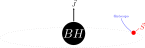
\includegraphics[scale=0.9]{images/solucion-en-kerr.pdf}
\caption[Solución helicoidal en Kerr]{Representación esquemática del sistema agujero negro-dipolo.}
\label{fig:7}
\end{figure}

Para responder esta pregunta procederemos a resolver las ecuaciones de movimiento \eqref{eq:69} y \eqref{eq:103}. Como estamos considerando órbitas circulares, y si por simplicidad suponemos que se encuentra en el plano ecuatorial, la velocidad de un observador co-móvil con el satélite es $u^{\mu} = \left[ u^t,0,0,u^{\phi} \right]$.

De \eqref{eq:68}, y la condición de normalización $u^{\mu}u_{\nu} = 1$, se obtiene que la 4-velocidad del satélite es
\begin{equation}
\label{eq:70}
u^{\mu} = \left [ \frac{\left(a^{2} + r^{2}\right)}{r\sqrt{a^{2} - 2 m r + r^{2}}}, \quad 0, \quad 0, \quad \frac{a}{r\sqrt{a^{2} - 2 m r + r^{2}}}\right ],
\end{equation}
y, definiendo $u_{\mu} := g_{\mu \nu} u^{\nu}$ tenemos que
\begin{equation}
\label{eq:71}
u_{\mu} = \left [ \frac{1}{r}\sqrt{a^{2} - 2 m r + r^{2}}, \quad 0, \quad 0, \quad -\frac{a}{r} \sqrt{a^{2} - 2 m r + r^{2}} \right ]
\end{equation}

Por otro lado, si definimos implícitamente el 4-vector de espín $S^{\mu}$ como 
\begin{equation}
S^{\mu} := -\frac{1}{2} \epsilon^{\mu \nu \rho \sigma} S_{\nu \rho} u_{\sigma},
\end{equation}
y tal que
\begin{equation}
S^{\mu \nu} = \epsilon^{\mu \nu \rho \sigma} S_{\rho} u_{\sigma},
\end{equation}
las ecuaciones de evolución para el vector de espín son
\begin{equation}
\label{eq:72}
\cd{S^{\mu}} = -S_{\nu} \cd{u^{\nu}} u^{\mu}.
\end{equation}

Reemplazando \eqref{eq:70} y \eqref{eq:71} en \eqref{eq:69} y \eqref{eq:72} se deducen las siguientes ecuaciones de movimiento para el momentum y el espín:
\begin{align}
\dot{p}^t(s) &= -\frac{m(R^2-a^2)}{R(a^2-2mR+R^2)^{3/2}} p^R(s),\\
\nonumber
\dot{p}^r(s) &= -\frac{\sqrt{a^2-2mR+R^2}}{R^5} \left( -a^{2}m p^t(s) - a m \left(a^{2} + R^{2}\right) p^{\phi}(s) + a \left(a^{2} m - R^{3}\right) p^{\phi}(s) \right.\\
& \quad \left. + m \left(a^{2} + R^{2} \right) p^t(s) \right),\\
\dot{p}^{\theta}(s) &= 0,\\
\dot{p}^{\phi}(s) &= -\frac{a(R-m)}{R(a^2-2mR+R^2)^{3/2}} p^r(s),\\
\dot{S}^t(s) &= -\frac{a^2}{R^2 \sqrt{a^2-2mR + R^2}} S^r(s),\\
\nonumber
\dot{S}^r(s) &= -\frac{\sqrt{a^2-2mR+R^2}}{R^5} \left( - a^{2} m S^t(s) - a m \left(a^{2} + R^{2}\right) S^{\phi}(s) + a \left(a^{2} m - R^{3}\right) S^{\phi}(s) \right.\\
& \quad \left. + m \left(a^{2} + R^{2} \right) S^t(s) \right),\\
\dot{S}^{\theta}(s) &= 0,\\
\dot{S}^{\phi}(s) &= \frac{a}{R\sqrt{a^2-2mR+R^2}} S^r(s).
\end{align} 

Las cuales son dos conjuntos de 4 ecuaciones ordinarias acopladas.

\section{Soluciones}

Luego de resolver las ecuaciones analíticamente, tenemos que la forma general de la solución es, para el caso del momentum, de la forma
\begin{align}
p^t(s) &= C_1 \alpha + \beta \left( C_2 e^{s \gamma} + C_3 e^{-s \gamma} \right),\\
p^r(s) &= \delta \left( C_2 e^{s \epsilon} - C_3 e^{-s \epsilon} \right),\\
p^{\theta}(s) &= C_4,\\
p^{\phi}(s) &= C_1 + C_2 e^{s \epsilon} + C_3 e^{-s \epsilon},
\end{align}
y para el espín es de la forma
\begin{align}
S^t(s) &= C_5 \eta + \kappa \left[ C_6 \cos\left(\frac{as}{R^2} \right) + C_7 \sin\left(\frac{as}{R^2} \right) \right],\\
S^r(s) &= C_6 \left[ \tau \sin\left(\frac{as}{R^2} \right) - \sigma \cos\left(\frac{as}{R^2} \right) \right] 
+ C_7 \left[ \tau \cos\left(\frac{as}{R^2} \right) - \sigma \sin\left(\frac{as}{R^2} \right) \right],\\
S^{\theta}(s) &= C_8,\\
S^{\phi}(s) &= C_5 + C_6 \cos\left(\frac{as}{R^2} \right) + C_7 \sin\left(\frac{as}{R^2} \right),
\end{align}
donde todos los elementos con letras griegas son factores que dependen de $(a,m,R)$ y no jugarán un rol importante en el futuro. Por otro lado, los coeficientes $C_1, \dots, C_8$ son constantes de integración y pueden ser calculadas reemplazando la solución en las condiciones que debe satisfacer.

La primera condición que imponemos es el hecho que al 4-velocidad y el 4-vector de espín deben ser ortogonales. De esta forma encontramos que $C_5=0$.

De \eqref{eq:44} y \eqref{eq:42} encontramos que las soluciones para el momentum y el espín deben estar relacionadas de forma que
\begin{equation}
p^{\mu} = M u^{\mu} + \epsilon^{\mu \nu \alpha \beta} \Gamma^{\rho}_{\nu \sigma} u_{\rho} u_{\alpha} S_{\beta} u^{\sigma},
\end{equation}
al reemplazar $\mu=r$ y $\mu=\theta$ se determina que $C_2 = C_3 = C_6 = C_7 = 0$, teniendo así que la forma general de las soluciones se reduce a 
\begin{align}
\label{eq:73}
p^{\mu} &= \left[ p^{\phi} \frac{a(m+R)}{m}, 0, 0, p^{\phi} \right],\\
\label{eq:74}
S^{\mu} &= \left[ 0,0,S^{\theta},0 \right],
\end{align}
donde se han renombrado las constantes $C_1$ y $C_4$ por $p^{\phi}$ y $S^{\theta}$ respectivamente.

Finalmente, reemplazando $\mu=t$ y $\mu=\phi$ se obtiene un sistema de dos ecuaciones lineales y dos incógnitas
\begin{align}
\frac{a p^{\phi}(m+R)}{m} &= \frac{S^{\theta} a^{3}}{R^{2} \sqrt{a^{2} - 2 m R + R^{2}}} - \frac{S^{\theta} a m}{R\sqrt{a^{2} - 2 m R + R^{2}}} + \frac{a^{3} p^{\phi}}{m R} + \frac{a p^{\phi} R}{m},\\
p^{\phi} &= \frac{S^{\theta} a^{2}}{R^{2}\sqrt{a^{2} - 2 m R + R^{2}}} - \frac{S^{\theta} m}{R\sqrt{a^{2} - 2 m R + R^{2}}} + \frac{a^{2} p^{\phi}}{m R}.
\end{align}

Dicho sistema es a un sistema compatible indeterminado, es decir, admite un conjunto infinito de soluciones descritas por
\begin{equation}
\label{eq:75}
S^{\theta} = - \frac{p^{\phi}R \sqrt{a^2 - 2mR +R^2}}{m}.
\end{equation}

Reemplazando \eqref{eq:75} en \eqref{eq:73} y \eqref{eq:74} encontramos que la solución exacta a las ecuaciones puede escribirse en términos de $p^{\phi}$ como
\begin{align}
p^{\mu} &= \left[ p^{\phi} \frac{a(m+r)}{m},\quad 0,\quad 0,\quad p^{\phi} \right],\\
S^{\mu} &= \left[0,\quad 0,\quad -\frac{p^{\phi} \sqrt{a^2+r^2-2mr}}{mr},\quad 0\right],
\end{align}
o, en términos de $S^{\theta}$, como
\begin{align}
\label{eq:76}
p^{\mu} &= \left [ - \frac{S^{\theta} a \left(m + r\right)}{r \sqrt{a^{2} - 2 m r + r^{2}} }, \quad 0, \quad 0, \quad - \frac{S^{\theta} m}{r\sqrt{a^{2} - 2 m r + r^{2}}}\right ],\\
\label{eq:77}
S^{\mu} &= \left [ 0, \quad 0, \quad S^{\theta}, \quad 0\right ].
\end{align}

Es importante destacar que la masa del satélite puede calcularse como
\begin{equation}
\label{eq:78}
M := p^{\mu} u_{\mu} = -\frac{S^{\theta}a}{r},
\end{equation}
y en términos de $M$, la solución puede escribirse como
\begin{align}
\label{eq:86}
p^{\mu} &= \left [ \frac{M \left(m + r\right)}{\sqrt{a^{2} - 2 m r + r^{2}}}, \quad 0, \quad 0, \quad \frac{M m}{a \sqrt{a^{2} - 2 m r + r^{2}}}\right ],\\
\label{eq:87}
S^{\mu} &= \left [ 0, \quad 0, \quad - \frac{Mr}{a}, \quad 0\right ].
\end{align}

\section{Propiedades de la solución}

De la solución podemos destacar varios puntos:
\begin{itemize}
\item[-] Los parámetros de la solución determinan una relación entre la masa y el espín del satélite, dicha relación nos da a entender que, por ejemplo, una vez fijado el valor del espín inmediatamente queda determinado el valor de la masa del satélite (o viceversa), de tal forma que se logre contrarrestar la atracción del agujero negro tal que la órbita se mantenga circular.
\item[-] La única dirección y sentido permitidos para el espín es ser antiparalelo a la rotación del agujero negro, esto es por el signo $-$ en \eqref{eq:78} que nos indica que el momento angular intrínseco del satélite debe ser opuesto a la rotación del agujero negro y el hecho de que la única componente no-nula para el espín es la componente $S^{\theta}$.
\end{itemize}

Es importante destacar que no es posible obtener el caso en la métrica de Schwarszchild a partir del resultado encontrado. Esto es por la suposición inicial al momento de plantear las ecuaciones de movimiento es que la velocidad angular del satélite es proporcional al parámetro rotacional del agujero negro, es decir $\omega \propto a$, y calcular el límite $a \rightarrow 0$ implica que $\omega = 0$, lo cual implicaría que la órbita no sería circular.

No obstante, es interesante hacer notar que si definimos la 4-fuerza sobre el satélite como
\begin{equation}
\label{eq:124}
F^{\mu} := M \cd{u^{\mu}} = \left[ 0, \frac{M(mR-a^2)}{R^3},0,0 \right],
\end{equation}
y si consideramos el caso asintótico, es decir $R \gg m $, entonces se puede deducir la ley de gravitación universal de Newton, esto cumple con el principio de correspondencia puesto que al encontrarse lejos del agujero negro no hay diferencia entre un agujero negro rotante y el campo gravitacional generado por una distribución de masa. Además, al ser una órbita circular en donde la único agente externo acutuando sobre el satélite tiene solo componente radial no-nula se puede ver que el satélite presenta un movimiento circular uniforme, ya que presenta una velocidad angular constante, logrando identificar así que \eqref{eq:124} corresponde a la fuerza centrípeta de la órbita.

Por último, es necesario agregar que la velocidad coordenada tangencial de la órbita es
\begin{equation}
v = \omega R = \frac{aR}{a^2 + R^2},
\end{equation}
lo cual en el mismo límite asintótico se reduce a
\begin{equation}
\label{eq:79}
v \approx \frac{a}{R},
\end{equation}
y reemplazando en \eqref{eq:78} se tiene que
\begin{align}
\nonumber
R &= -\frac{S^{\theta}a}{M},\\
\nonumber
&= -\frac{S^{\theta}aR}{MR},\\
\label{eq:80}
&= -\frac{vS}{M},
\end{align}
donde $S = R S^{\theta}$ y es el módulo del espín (que coincide con el valor de la componente $z$ en un plano cartesiano).

Podemos agregar que \eqref{eq:80} representa la misma condición encontrada en \cite{Costa-Herdeiro-Natario-Zilhao} para el problema análogo en el espaciotiempo de Minkowski en coordenadas cartesianas mostrando así que la solución obtenida en \eqref{eq:86} y \eqref{eq:87} se reduce asintóticamente al caso en la métrica plana.						%Cap�tulo de las soliciones
\newpage
\chapter{Conclusiones y trabajos futuros}

En la presente tesis se ha estudiado la analogía gravitoelectromagnética propuesta por Costa \& Herdeiro, en la cual se ha extendido su análisis con el fin de introducir órdenes superiores en la expansión multipolar para comparar de una forma más general ambas teorías, además de estudiar y resolver casos particulares como el presentado en el capítulo \ref{cap:4}, de esta forma las principales conclusiones son:
\begin{itemize}
\item La discusión realizada en \cite{Costa-Herdeiro} no puede ser extendida a orden cuadrupolar, esto es por que a dicho orden es necesaria la información completa del tensor de Riemann para determinar las ecuaciones de movimiento de los objetos en cuestión, y dicho tensor no puede ser reconstruido completamente utilizando los tensores de marea, teniendo así que la analogía propuesta basada en tensores de marea no permite una exacta correspondencia entre ambas teorías como sí ocurría en el caso dipolar.
\item A partir de la solución obtenida en el capítulo \ref{cap:4} se pueden deducir las características que debe satisfacer un giróscopo que mantiene una órbita circular ecuatorial alrededor de un agujero negro rotante. Estas características determinan el valor del espín, y evidenecian una directa relación entre la magnitud del espín y la masa del giróscopo, la cual nos da a entender que para un giróscopo de masa $M$ existirá solo un valor de espín $S$ tal que sea compatible con la órbita previamente establecida.
\end{itemize}

No obstante, a lo largo de este trabajo se han abierto algunos problemas los cuales pueden ser tratados en trabajos futuros, como lo son:
\begin{itemize}
\item Obtener una solución similar al problema resuelto en el capítulo \ref{cap:4} pero con una velocidad angular arbitraria. Esto entregaría una solución más general a dicho problema a costa de hacer no-nulo el lado derecho de las ecuaciones de movimiento en \eqref{eq:66}, puesto que permitiría aumentar los grados de libertad del sistema al no existir una relación previamente fijada entre las coordenadas $u^t$ y $u^{\phi}$.
\item Realizar un análisis detallado para la estabilidad de la órbita. Es decir, a partir de la solución obtenida en la presente tesis, considerar una pequeña perturbación dependiente del tiempo, y a partir de las ecuaciones de movimiento, determinar la evolución de la perturbación.
\end{itemize}

\appendix
\chapter{Notación y convenciones}
\label{ape:convenciones}

En el desarrollo de la presente tesis se utilizó el siguiente conjunto de notaciones y convenciones:

\begin{itemize}
\item Las coordenadas de los elementos se denotan como $x^{\mu}=\left( x^0, x^1, x^2, x^3 \right)$, donde $x^0$ corresponde a la coordenada temporal.
\item Usamos la convención $\eta_{\mu \nu} = \mathrm{diag}(1,-1,-1,-1)$.
\item Se define el tensor totalmente antisimétrico de Levi-Civita como $\epsilon_{\mu \nu \rho \sigma} := \sqrt{-g} \hat{\epsilon}_{\mu \nu \rho \sigma}$ y tal que $\hat{\epsilon}_{\mu \nu \rho \sigma}$ es el símbolo totalmente antisimétrico de Levi-Civita donde $\hat{\epsilon}_{0123} = \hat{\epsilon}^{0123} = 1$.

Además, se define el tensor contravariante $\epsilon^{\mu \nu \rho \sigma} := g^{\mu \alpha} g^{\nu \beta} g^{\rho \gamma} g^{\sigma \delta} \epsilon_{\alpha \beta \gamma \delta} = \frac{1}{\sqrt{-g}} \hat{\epsilon}^{\mu \nu \rho \sigma}$.

El tensor de Levi-Civita satisface las siguientes propiedades
\begin{align*}
\epsilon^{\mu \nu \rho \sigma} \epsilon_{\mu \nu \rho \sigma} &= -24,\\
\epsilon^{\mu \nu \rho \sigma} \epsilon_{\alpha \nu \rho \sigma} &= -6 \delta^{\mu}_{\ \alpha},\\
\epsilon^{\mu \nu \rho \sigma} \epsilon_{\alpha \beta \rho \sigma} &= -2 \left( \delta^{\mu}_{\ \alpha} \delta^{\nu}_{\ \beta} - \delta^{\mu}_{\ \beta} \delta^{\nu}_{\ \alpha} \right),\\
\epsilon^{\mu \nu \rho \sigma} \epsilon_{\alpha \beta \gamma \sigma} &= - 2\left( \delta^{\mu}_{\ \alpha}\delta^{[\nu}_{\ \beta}\delta^{\rho]}_{\ \gamma} + \delta^{\mu}_{\ \gamma}\delta^{[\nu}_{\ \alpha}\delta^{\rho]}_{\ \beta} + \delta^{\mu}_{\ \beta}\delta^{[\nu}_{\ \gamma}\delta^{\rho]}_{\ \alpha} \right),
\end{align*}
\item Usamos letras del alfabeto griego $\mu, \nu, \rho, \dots$ para referirnos a índices espaciotemporales 4-dimensionales que varían de 0 a 3, y letras del abecedario latino $i, j, k, \dots$ para referirnos a índices espaciales que varían de 1 a 3.
\item Se utiliza la convención de suma de Einstein, es decir, cuando dos índices se encuentra repetidos en el mismo término, existe una sumatoria de 0 a 3 o de 1 a 3 dependiendo si son índices del alfabeto griego o latino.
\item Se utilizan unidades gausiannas\footnote{\url{https://en.wikipedia.org/wiki/Gaussian_units}} con $c=1$.
\item Las derivadas parciales son $\partial_{\mu} := \partial / \partial x^{\mu}$.
\item Los símbolos de Christoffel de segunda especie están definidos como
\begin{equation}
\Gamma^{\mu}_{\rho \sigma} := \frac{1}{2} g^{\mu \gamma} \left( \partial_{\rho} g_{\gamma \sigma} + \partial_{\sigma} g_{\gamma \rho} - \partial_{\gamma} g_{\rho \sigma} \right).
\end{equation}
\item El tensor de curvatura de Riemann definido como 
\begin{equation}
R_{\mu \nu \beta}^{\ \ \ \ \alpha} =-R^{\alpha}_{\ \beta \mu \nu} = \partial_{\mu} \Gamma^{\alpha}_{\beta \nu} - \partial_{\nu} \Gamma^{\alpha}_{\beta \mu} + \Gamma^{\alpha}_{\delta \mu} \Gamma^{\delta}_{\beta \nu} - \Gamma^{\alpha}_{\delta \nu} \Gamma^{\delta}_{\beta \mu}.
\end{equation}
\item El tensor de Ricci está definido como
\begin{equation}
R_{\mu \nu} := g^{\alpha \beta} R_{\alpha \mu \beta \nu}.
\end{equation}
\item El escalar de curvatura está definido como 
\begin{equation}
R := g^{\mu \nu} R_{\mu \nu}.
\end{equation}
\item La densidad tensorial de energía-momentum $\tilde{T}^{\mu \nu}$ se define como un tensor de rango $\left(^2_0 \right)$ y peso $-1$, es decir que transforma bajo transformaciones generales de coordenadas como 
\begin{equation}
\tilde{T}^{'\mu \nu} =  \frac{\partial x^{\mu}}{\partial x^{\alpha}} \frac{\partial x^{\nu}}{\partial x^{\beta}} \tilde{T}^{\alpha \beta} | J |^{-1},
\end{equation}
donde $J$ es la matriz jacobiana, y tal que
\begin{equation}
\tilde{T}^{\mu \nu} := \sqrt{-g} T^{\mu \nu}.
\end{equation}
\end{itemize}
\chapter{Ecuaciones de movimiento para una part\'icula monopolar}
\label{ape:1}

Para demostrar la identidad mostrada en \eqref{eq:88} es \'util notar que el argumento de la funci\'on delta de Dirac es $\delta_{(4)}=\delta_{(4)}(x^{\mu}-X^{\mu})$, lo cual permite tratar de igual forma las componentes del espaciotiempo $x^{\mu}$ con las componentes de la curva de referencia $X^{\mu}$, de esta forma tenemos que
\begin{align}
\nonumber
\int_{-\infty}^{+\infty} \mathrm{d}s \nabla_{\nu} [u^{\nu} T^{\mu_1 \mu_2 \dots} \delta_{(4)}] &=
\int_{-\infty}^{+\infty} \mathrm{d}s \left\{ u^{\nu} \nabla_{\nu} \left( T^{\mu_1 \mu_2 \dots} \delta_{(4)} \right)  \right\}\\
\nonumber
&= \int_{-\infty}^{+\infty} \mathrm{d}s \cd{T^{\mu_1 \mu_2 \dots}} \delta_{(4)} + \int_{-\infty}^{+\infty} \mathrm{d}s T^{\mu_1 \mu_2 \dots} \nabla_{\nu} \left( u^{\nu} \delta_{(4)} \right)\\
\label{eq:89}
&= \int_{-\infty}^{+\infty} \mathrm{d}s \cd{T^{\mu_1 \mu_2 \dots}} \delta_{(4)} + \int_{-\infty}^{+\infty} \mathrm{d}s T^{\mu_1 \mu_2 \dots} \left( u^{\nu} \nabla_{\nu} \delta_{(4)} + \delta_{(4)} \nabla_{\nu} u^{\nu} \right).
\end{align}

Es importante notar que
\begin{align}
u^{\nu} \nabla_{\nu} \delta_{(4)} + \delta_{(4)} \nabla_{\nu} u^{\nu} &= u^{\nu} \partial_{\nu} \delta_{(4)} - \Gamma^{\mu}_{\mu \nu} u^{\nu} \delta_{(4)} + \delta_{(4)} \partial_{\nu} u^{\nu} + \Gamma^{\nu}_{\nu \mu} u^{\nu} u^{\mu} \delta_{(4)} \nonumber \\
&= u^{\nu} \partial_{\nu} \delta_{(4)} + \delta_{(4)} \partial_{\nu} u^{\nu} \nonumber \\
\label{eq:90}
&= \partial_{\mu} \left( u^{\mu} \delta_{(4)} \right).
\end{align}

Reemplazando \eqref{eq:90} en \eqref{eq:89} se obtiene que
\begin{align}
\int_{-\infty}^{+\infty} \mathrm{d}s \nabla_{\nu} [u^{\nu} T^{\mu_1 \mu_2 \dots} \delta_{(4)}] &= \int_{-\infty}^{+\infty} \mathrm{d}s \cd{T^{\mu_1 \mu_2 \dots}} \delta_{(4)} + \int_{-\infty}^{+\infty} \mathrm{d}s T^{\mu_1 \mu_2 \dots} \partial_{\mu} \left( u^{\mu} \delta_{(4)} \right).
\end{align}

Como el tensor de energ\'ia-momentum esta evaluado sobre la curva de referencia, la cual esta descrita por el parámetro $s$, al igual que la 4-velocidad, entonces podemos reescribir la ecuaci\'on anterior como
\begin{equation}
\label{eq:91}
\int_{-\infty}^{+\infty} \mathrm{d}s \nabla_{\nu} [u^{\nu} T^{\mu_1 \mu_2 \dots} \delta_{(4)}] = \int_{-\infty}^{+\infty} \mathrm{d}s \cd{T^{\mu_1 \mu_2 \dots}} \delta_{(4)} + \int_{-\infty}^{+\infty} \mathrm{d}s u^{\mu}  \partial_{\mu} \left( T^{\mu_1 \mu_2 \dots} \delta_{(4)} \right),
\end{equation}
y recordando que las integrales son respecto al par\'ametro de la curva, tenemos que el segundo t\'ermino al lado derecho de \eqref{eq:91} es un t\'ermino de borde, as\'i
\begin{equation}
\int_{-\infty}^{+\infty} \mathrm{d}s \nabla_{\nu} [u^{\nu} T^{\mu_1 \mu_2 \dots} \delta_{(4)}] = \int_{-\infty}^{+\infty} \mathrm{d}s \cd{T^{\mu_1 \mu_2 \dots}} \delta_{(4)}.
\end{equation}
\chapter{Orden menor en la expansi\'on para una part\'icula monopolo-dipolo}
\label{ape:3}

Para obtener \eqref{eq:43} usaremos el teorema \ref{teo:2} en \eqref{eq:37}, de donde se obtiene que del orden m\'as bajo
\begin{equation}
\label{eq:94}
\frac{\delta^2}{\mathrm{d}s^2} (t^{\gamma \rho \nu} u_{\gamma}u_{\rho}) + \cd{} (t^{\gamma \nu} u_{\gamma} - 2\cd{u_{\gamma}} u_{\rho} t^{(\gamma \rho) \nu}) + \frac{1}{2} R^{\ \ \ \ \nu}_{\mu \gamma \delta} (2 u^{\mu} u_{\rho} t^{\hat{\gamma} \rho \delta} + t^{\hat{\gamma} \hat{\mu} \delta}) = 0.
\end{equation}

Trabajando cada t\'ermino por separado se tiene que
\begin{align}
\label{eq:95}
\cd{} \left( t^{\gamma \sigma \nu} u_{\gamma} u_{\sigma} \right) &= \cd{u_{\sigma}} \des{1}{t}^{\sigma \nu} + u_{\gamma} \cd{\des{1}{t}^{\sigma \nu}},\\
\label{eq:96}
t^{\gamma \nu} u_{\gamma} &= \ \des{0}{o}^{\nu} + \des{0}{t}^{\nu} u^{\nu},\\
\label{eq:97}
\cd{u_{\gamma}} u_{\sigma} t^{\gamma \sigma \nu} &= \cd{u_{\gamma}} \left( \des{1}{o}^{\gamma \nu} + \des{1}{o}^{\gamma} u^{\nu} \right),\\
\label{eq:98}
\cd{u_{\gamma}} u_{\sigma} t^{\sigma \gamma \nu} &= \cd{u_{\gamma}} \des{1}{t}^{\gamma \nu}.\\
\label{eq:100}
2 t^{\hat{\gamma} \sigma \rho} u^{\mu} u_{\sigma} &= 2u^{\mu} \left( \des{1}{o}^{\gamma \rho} + \des{1}{o}^{\gamma} u^{\rho} \right),\\
\label{eq:101}
t^{\hat{\gamma} \hat{\mu} \rho} &= \ \des{1}{o}^{\gamma \rho \mu} + \des{1}{o}^{\gamma \mu} u^{\rho}
\end{align}

Reemplazando \eqref{eq:95}, \eqref{eq:96}, \eqref{eq:97} y \eqref{eq:98} en los primeros dos t\'erminos de \eqref{eq:94} se obtiene que
\begin{align}
& \frac{\delta^2}{\mathrm{d}s^2} (t^{\gamma \rho \nu} u_{\gamma}u_{\rho}) + \cd{} (t^{\gamma \nu} u_{\gamma} - 2\cd{u_{\gamma}} u_{\rho} t^{(\gamma \rho) \nu}) \nonumber\\
& \quad = \cd{} \left( \cd{} \left( t^{\gamma \sigma \nu} u_{\gamma \sigma} \right) + t^{\gamma \nu} u_{\gamma} - \cd{u_{\gamma}} u_{\sigma} t^{\gamma \sigma \nu} - \cd{u_{\gamma}} u_{\sigma} t^{\sigma \gamma \nu} \right) \nonumber \\
\label{eq:99}
& \quad = \cd{} \left( u_{\gamma} \cd{} \des{1}{t}^{\gamma \nu} + \des{0}{o}^{\nu} + \des{0}{t} u^{\nu} - \cd{u_{\gamma}} \des{1}{o}^{\gamma \nu} - \cd{\gamma} \des{1}{o}^{\gamma}u^{\nu} \right).
\end{align}

Y reemplazando \eqref{eq:100} y \eqref{eq:101} en el tercer t\'ermino de \eqref{eq:37} se obtiene que
\begin{equation}
\label{eq:102}
 \frac{1}{2} R^{\ \ \ \ \nu}_{\mu \gamma \delta} (2 u^{\mu} u_{\rho} t^{\hat{\gamma} \rho \delta} + t^{\hat{\gamma} \hat{\mu} \delta}) = \frac{1}{2} R^{\ \ \ \ \nu}_{\mu \gamma \rho} \left[ 2u^{\mu}(\des{1}{o}^{\gamma \rho} + \des{1}{o}^{\gamma} u^{\rho}) + \des{1}{o}^{\gamma \mu \rho} + \des{1}{o}^{\gamma \mu}  u^{\rho}  \right],
\end{equation}
luego, de \eqref{eq:99} y \eqref{eq:102} se obtiene \eqref{eq:43}.
\chapter{Ecuaciones de movimiento para una partícula monopolo-dipolo}
\label{ape:2}

Para obtener \eqref{eq:82} trabajaremos el primer t\'ermino de \eqref{eq:43}, as\'i
\begin{align}
& \cd{} \left( u_{\gamma} \cd{} \des{1}{t}^{\gamma \nu} + \des{0}{o}^{\nu} + \des{0}{t} u^{\nu} - \cd{u_{\gamma}} \des{1}{o}^{\gamma \nu} - \cd{\gamma} \des{1}{o}^{\gamma}u^{\nu} \right) \nonumber\\
&\quad = \cd{} \left[ u_{\gamma} \des{1}{t}^{\gamma \nu} -  \rho^{\nu}_{\ \delta} u_{\gamma} \cd{} \left( \des{1}{o}^{\delta \gamma} + \des{1}{o}^{\delta} u^{\gamma} + \des{1}{t}^{\delta \gamma} \right) + \des{0}{t} u^{\nu} - \cd{u_{\gamma}} \des{1}{o}^{\gamma \nu} -  \cd{u_{\gamma}} \des{0}{o}^{\gamma} u^{\nu} \right] \nonumber \\
&\quad = \cd{}  \left[ u^{\nu} u_{\gamma} u_{\sigma} \cd{} \left( \des{1}{o}^{\gamma} u^{\sigma} \right) + u_{\gamma} u_{\sigma} u^{\nu} \cd{} \des{1}{t}^{\gamma \sigma} + \des{0}{t} u^{\nu} - u_{\gamma} \cd{\des{1}{o}^{\nu \gamma}} - u_{\gamma} \cd{\des{1}{o}^{\nu} u^{\gamma}} - \cd{u_{\gamma}} \des{1}{o}^{\gamma \nu} \right. \nonumber \\
&\qquad \left. - \cd{u_{\gamma}} \des{1}{o}^{\gamma} u^{\nu} \right] \nonumber \\
&\quad = \cd{}  \left[  -u^{\nu} u_{\gamma} \cd{u_{\sigma} \des{1}{S}^{\gamma \sigma}} + u_{\gamma} u_{\sigma} u^{\nu} \cd{\des{1}{t}^{\gamma \sigma}} + \des{0}{t} u^{\nu} + u_{\gamma} \left(  \frac{1}{2} \des{1}{S}^{\nu \gamma} + u_{\sigma} \des{1}{S}^{\sigma [\nu} u^{\gamma]} \right) \right. \nonumber \\
&\qquad \left. + \cd{} \left( u_{\gamma} \des{1}{S}^{\nu \gamma} \right) + \frac{1}{2} \cd{u_{\gamma}} \left( \des{1}{S}^{\gamma \nu} + 2u_{\sigma} \des{1}{S}^{\sigma [\gamma} u^{\nu]} \right) + \cd{u_{\gamma}} u_{\sigma} \des{1}{S}^{\gamma \sigma} u^{\nu} \right] \nonumber\\
&\quad = \cd{} \left[ u^{\nu} u_{\gamma} \cd{u_{\sigma}} \des{1}{S}^{\sigma \gamma} + u_{\gamma} u_{\sigma} \cd{\des{1}{t}^{\gamma \sigma}} u^{\nu} + \des{0}{t} u^{\nu} + \frac{1}{2} \cd{} \left(       u_{\gamma} \des{1}{S}^{\gamma \nu} \right) - \frac{1}{2} u_{\sigma} \cd{} \left( u_{\gamma} u^{\nu} \des{1}{S}^{\gamma \sigma} \right) \right. \nonumber \\
&\qquad \left. + \cd{}\left( u_{\gamma} \des{1}{S}^{\nu \gamma} \right) + \frac{1}{2} u_{\gamma} \cd{\des{1}{S}^{\nu \gamma}} + \frac{1}{2} \des{1}{S}^{\gamma \nu} \cd{u_{\gamma}} + \frac{1}{2} \cd{u_{\gamma}} u_{\sigma} \des{1}{S}^{\gamma \sigma} u^{\nu} \right] \nonumber
\end{align}
\newpage

\begin{align}
&\quad = \cd{} \left[ u^{\nu} u_{\gamma} \cd{u_{\sigma}} \des{1}{S}^{\sigma \gamma} + u_{\gamma} u_{\sigma} \cd{\des{1}{t}^{\gamma \sigma}} u^{\nu} + \des{0}{t} u^{\nu} - \frac{1}{2} \cd{} \left(       u_{\gamma} \des{1}{S}^{\nu \gamma} \right) - \frac{1}{2} u_{\sigma} \cd{} \left( u_{\gamma} u^{\nu} \des{1}{S}^{\gamma \sigma} \right) \right. \nonumber \\
&\qquad \left. + \cd{}\left( u_{\gamma} \des{1}{S}^{\nu \gamma} \right) + \frac{1}{2} u_{\gamma} \cd{\des{1}{S}^{\nu \gamma}} - \frac{1}{2} \des{1}{S}^{\nu \gamma} \cd{u_{\gamma}} + \frac{1}{2} \cd{u_{\gamma}} u_{\sigma} \des{1}{S}^{\gamma \sigma} u^{\nu} \right] \nonumber\\
&\quad = \cd{} \left[ u^{\nu} u_{\gamma} \cd{u_{\sigma}} \des{1}{S}^{\sigma \gamma} + u_{\gamma} u_{\sigma} \cd{\des{1}{t}^{\gamma \sigma}} u^{\nu} + \des{0}{t} u^{\nu} + \frac{1}{2} \cd{} \left(       u_{\gamma} \des{1}{S}^{\nu \gamma} \right) - \frac{1}{2} u_{\sigma} \cd{} \left( u_{\gamma} u^{\nu} \des{1}{S}^{\gamma \sigma} \right) \right. \nonumber \\
&\qquad \left. +\frac{1}{2} u_{\gamma} \cd{\des{1}{S}^{\nu \gamma}} - \frac{1}{2} \des{1}{S}^{\nu \gamma} \cd{u_{\gamma}} + \frac{1}{2} \cd{u_{\gamma}} u_{\sigma} \des{1}{S}^{\gamma \sigma} u^{\nu} \right] \nonumber\\
& \qquad= \cd{} \left[ \left( \des{0}{t} - u_{\gamma} \cd{u_{\rho}} \des{1}{S}^{\gamma \rho} + u_{\gamma} u_{\rho} \cd{\des{1}{t}^{\gamma \rho}} \right) u^{\mu} + u_{\gamma} \cd{} \des{1}{S}^{\mu \gamma} \right] \nonumber\\
\label{eq:92}
&\quad = \cd{p^{\nu}}.
\end{align}

Por otro lado, si trabajamos el segundo t\'ermino en \eqref{eq:43} se tiene que
\begin{align}
& \frac{1}{2} R^{\ \ \ \ \nu}_{\mu \gamma \rho} \left[ 2u^{\mu}(\des{1}{o}^{\gamma \rho} + \des{1}{o}^{\gamma} u^{\rho}) + \des{1}{o}^{\gamma \mu \rho} + \des{1}{o}^{\gamma \mu}  u^{\rho}  \right] \nonumber \\
& \quad = \frac{1}{2} R^{\ \ \ \ \nu}_{\mu \gamma \rho} \left[ 2 u^{\mu} \left( -\frac{1}{2} \des{1}{S}^{\gamma \rho} - \frac{1}{2} u_{\sigma} \des{1}{S}^{\sigma \gamma} u^{\rho} + \frac{1}{2} u_{\sigma} \des{1}{S}^{\sigma \rho} u^{\gamma} - u_{\sigma} \des{1}{S}^{\gamma \sigma} u^{\rho} \right) \right. \nonumber \\
&\qquad \left. - \frac{1}{2} \des{1}{S}^{\gamma \mu} u^{\rho} - \frac{1}{2} u_{\sigma} \des{1}{S}^{\sigma \gamma} u^{\mu} u^{\rho} + \frac{1}{2} u_{\sigma} \des{1}{S}^{\sigma \mu} u^{\gamma} u^{\rho}  \right] \nonumber\\
& \quad = - \frac{1}{2} R^{\ \ \ \ \nu}_{\mu \gamma \rho} \des{1}{S}^{\gamma \rho} u^{\mu} - \frac{1}{4} R^{\ \ \ \ \nu}_{\mu \gamma \rho} \des{1}{S}^{\gamma \mu} u^{\rho}, \nonumber
\end{align}
y usando que $R_{[\mu \nu \gamma]}^{\ \ \ \ \sigma} = 0$, se obtiene que
\begin{equation}
\label{eq:93}
\frac{1}{2} R^{\ \ \ \ \nu}_{\mu \gamma \rho} \left[ 2u^{\mu}(\des{1}{o}^{\gamma \rho} + \des{1}{o}^{\gamma} u^{\rho}) + \des{1}{o}^{\gamma \mu \rho} + \des{1}{o}^{\gamma \mu}  u^{\rho} \right] = \frac{1}{2} R^{\ \ \ \ \nu}_{\gamma \mu \rho} \des{1}{S}^{\gamma \mu} u^{\rho}.
\end{equation}

De esta forma, usando \eqref{eq:92} y \eqref{eq:93} se obtiene directamente \eqref{eq:82}.



\chapter{Cantidades conservadas y evoluci\'on del esp\'in}
\label{ape:6}

Para demostrar \eqref{eq:45} usaremos la definición del 4-momentum y la evolución de este.

Reemplazando \eqref{eq:44} en \eqref{eq:82} se obtiene que
\begin{equation}
\cd{} \left[ \des{1}{m} u^{\mu} + u_{\gamma} \cd{} \des{1}{S}^{\mu \gamma} \right] = -\frac{1}{2} R^{\ \ \ \ \mu}_{\nu \gamma \rho} \des{1}{S}^{\mu \gamma} u^{\rho}.
\end{equation}

Multiplicando con $u_{\mu}$ el lado derecho se anula, quedando
\begin{equation}
u_{\mu} \cd{} \left[ \des{1}{m} u^{\mu} + u_{\gamma} \cd{} \des{1}{S}^{\mu \gamma} \right] = 0.
\end{equation}

Expandiendo y despejando el valor de la derivada de la masa obtenemos que
\begin{equation}
\cd{\des{1}{m}} = u_{\nu} \cd{u_{\gamma}} \cd{} \des{1}{S}^{\nu \gamma} = \cd{u_{\gamma}} \cd{} \left( u_{\nu} \des{1}{S}^{\nu \gamma} \right).
\end{equation}

Para demostrar \eqref{eq:103} a partir de la definición del 4-momentum se puede ver que
\begin{equation}
\des{1}{p}^{\mu} u^{\nu} = \ \des{1}{m} u^{\mu} u^{\nu} + u_{\gamma}  u^{\nu} \cd{} \des{1}{S}^{\mu \gamma},
\end{equation}
lo cual si antisimetrizamos se convierte en
\begin{equation}
\des{1}{p}^{\mu} u^{\nu} - \des{1}{p}^{\nu} u^{\mu} = u_{\gamma}  u^{\nu} \cd{} \des{1}{S}^{\mu \gamma} - u_{\gamma}  u^{\mu} \cd{} \des{1}{S}^{\nu \gamma},
\end{equation}
y de \eqref{eq:83} se obtiene
\begin{equation}
\label{eq:113}
\cd{} \des{1}{S}^{\mu \nu} = 2 \des{1}{p}^{[\mu} u^{\nu]}.
\end{equation}

Por último, también podemos demostrar la conservación de \eqref{eq:46} y \eqref{eq:47}. Es inmediato notar que de \eqref{eq:47} y \eqref{eq:104} se deduce que
\begin{equation}
\cd{S^2} = 4 S_{\mu \nu} p^{[ \mu} u^{\nu]},
\end{equation}
de donde es inmediato ver que asumiendo cualquiera de las dos condiciones, ya sea la de Mathisson-Pirani o de Tulczyjew, dicha cantidad se conserva a lo largo de la curva.

Por último, podemos asegurar la conservación \eqref{eq:46} de un calculo previo. Sabemos que
\begin{equation}
\label{eq:104}
\cd{\bar{m}} = \frac{1}{2\bar{m}} \cd{p^{\mu} p_{\mu}} \quad \Rightarrow \quad \bar{m} \cd{\bar{m}} = p^{\mu} \cd{p_{\mu}}.
\end{equation}

Además podemos ver que al multiplicar \eqref{eq:113} con $p_{\mu}$ se obtiene que
\begin{equation}
p_{\mu} \cd{S^{\mu \nu}} = \bar{m}^2 u^{\nu} - m p^{\nu},
\end{equation}
lo cual, al multiplicar por $\delta p_{\nu} / \mathrm{d}s$ se transforma en
\begin{equation}
\cd{p_{\nu}} p_{\mu} \cd{S^{\mu \nu}} = \bar{m}^2 u^{\nu} \cd{p_{\nu}} - mp^{\nu} \cd{p_{\nu}},
\end{equation}
y al reemplazar \eqref{eq:82} se deduce que
\begin{equation}
\label{eq:105}
m \bar{m} \cd{\bar{m}} = - p_{\mu} \cd{p_{\nu}} \cd{S^{\mu \nu}}.
\end{equation}

Finalmente al reemplazar \eqref{eq:105} en \eqref{eq:104}, vemos que al utilizar la condición suplementaria de Tulczyjew, la masa $\bar{m}$ es una cantidad que se conserva a lo largo de la curva.
\chapter{Transformación inversa para los tensores de marea}
\label{ape:4}

Para demostrar las ecuaciones \eqref{eq:52} tenemos que a partir de la definición \eqref{eq:51} se puede construir que
\begin{align}
\epsilon_{\alpha \beta \mu \sigma} \mathtt{B}^{\mu}_{\ \gamma} u^{\sigma} &= \frac{1}{2} \epsilon_{\alpha \beta \mu \sigma} \epsilon^{\delta \lambda \rho \mu} \partial_{\gamma} F_{\rho \lambda} u_{\delta} u^{\sigma}\\
&= \partial_{\gamma} F_{\mu \nu} + 2u_{[\alpha} \mathtt{E_{\beta] \gamma}},
\end{align}
de donde se puede deducir que
\begin{equation}
\partial_{\gamma} F_{\mu \nu} =  \epsilon_{\alpha \beta \mu \sigma} \mathtt{B}^{\mu}_{\ \gamma} u^{\sigma} - 2u_{[\alpha} \mathtt{E_{\beta] \gamma}}.
\end{equation}

Para el caso gravitacional tenemos que, de forma similar, se puede construir que
\begin{align}
\epsilon_{\alpha \beta \mu \sigma} \mathbb{H}^{\mu}_{\ \gamma} u^{\sigma} &= \frac{1}{2} \epsilon_{\alpha \beta \mu \sigma} \epsilon^{\rho \lambda \mu \delta} R_{\rho \lambda \gamma \xi} u_{\delta} u^{\xi} u^{\sigma}\\
&= R_{\alpha \beta \xi \gamma} u^{\xi} + 2u_{[\alpha} \mathbb{E}_{\beta] \gamma},
\end{align}
de donde se deduce que
\begin{equation}
R_{\alpha \beta \gamma \xi} u^{\xi} = \epsilon_{\alpha \beta \mu \sigma} \mathbb{H}^{\mu}_{\ \gamma} u^{\sigma} - 2u_{[\alpha} \mathbb{E}_{\beta] \gamma}.
\end{equation}

%\chapter{Script}
\label{ape:5}

\begin{minted}{python}
from numpy import *
from GRpy.all import *

t, x0, r, th, phi = symbols('t, x^0, r, theta, varphi', 
positive=True, real=True)
m,a = symbols('m,a', positive = True)
ut, uphi = symbols('u_t, u_phi', real=True)
p3, sp2 = symbols(r'p^{\phi}, S^{\theta}', real=True)
M = Symbol('M', real=True)

s = Symbol('s', real=True)

pt = Function(r'p^t')(s)
pr = Function(r'p^r')(s)
ptheta = Function(r'p^{\theta}')(s)
pphi = Function(r'p^{\phi}')(s)

st = Function(r'S^t')(s)
sr = Function(r'S^r')(s)
stheta = Function(r'S^{\theta}')(s)
sphi = Function(r'S^{\phi}')(s)

sigma = r**2 + (a*cos(th))**2
delta = r**2 - 2*m*r + a**2

g = Metric((x0, r, th, phi))
g[-0,-0] = (1-(2*m*r/sigma))
g[-0,-1] = 0
g[-0,-2] = 0
g[-0,-3] = (2*a*m*r*sin(th)**2)/sigma
g[-1,-0] = 0
g[-1,-1] = -sigma/delta
g[-1,-2] = 0
g[-1,-3] = 0
g[-2,-0] = 0
g[-2,-1] = 0
g[-2,-2] = -sigma
g[-2,-3] = 0
g[-3,-0] = (2*a*m*r*sin(th)**2)/sigma
g[-3,-1] = 0
g[-3,-2] = 0
g[-3,-3] = -(r**2 +a**2 + (2*a**2*m*r*sin(th)**2)/sigma)*sin(th)**2

ginv = g.invert()
chris = Christoffel(g)

def dw(A,mu):
    downvector=0
    for nu in range(4):
        downvector += g.components[(-mu,-nu)]*A[nu]
    
    return simplify(downvector.subs(th,pi/2))

def down(A):
    return [dw(A,mu) for mu in range(4)]

sup=[st,sr,stheta,sphi]
pup=[pt,pr,ptheta,pphi]

uphi=a/(a**2+r**2)*ut
uupnonorm=[ut,0,0,uphi]

N=0
for i in range(4):
    for j in range(4):
        N += g.components[(-i,-j)]*uupnonorm[i]*uupnonorm[j]
        
eq=1-N.subs(th,pi/2)

utnorm=solve(eq,ut)[1]
uphinorm=a/(a**2+r**2)*utnorm
uup=[utnorm,0,0,uphinorm]
udown=down(uup)

def ch(mu):
    ch=0
    for i in range(4):
        for j in range(4):
            ch += chris.components[(mu,-i,-j)]*uup[i]*pup[j]
        
    return ch

def dpmu(mu):
    A=simplify(ch(mu).subs(th,pi/2))
    return diff(pup[mu],s)+A

dpmu=[dpmu(0),dpmu(1),dpmu(2),dpmu(3)]

sdown=down(sup)

c2=0
for i in range(4):
    for j in range(4):
        for k in range(4):
            c2 += chris.components[(i,-j,-k)]*sdown[i]*uup[j]*uup[k]
            
def c3(mu):
    c=0
    for i in range(4):
        for j in range(4):
            c += chris.components[(mu,-i,-j)]*sup[i]*uup[j]
    
    return c

def dsmu(mu):
    A=c3(mu)+uup[mu]*c2
    B=simplify(A.subs(th,pi/2))
    return diff(sup[mu],s)+B
    
dsmu=[dsmu(0),dsmu(1),dsmu(2),dsmu(3)]

dpmu2=[dpmu[0],dpmu[1],dpmu[3]]
psol=dsolve(dpmu2)
dsmu2=[dsmu[0],dsmu[1],dsmu[3]]
ssol=dsolve(dsmu2)

supsol = [ssol[0].rhs,ssol[1].rhs,sp2,ssol[2].rhs]

condicion=0
for i in range(4):
    condicion += supsol[i]*udown[i]

print('la condicion a satisfacer es:',simplify(condicion))

pupsol = [psol[0].rhs, psol[1].rhs ,p3, psol[2].rhs]
sdownsol=down(supsol)

def lcup(i,j,k,l):
    return LeviCivita(i,j,k,l)/(r**2)

def termino(mu):
    termino=0
for nu in range(4):
for alpha in range(4):
for beta in range(4):
for sigma in range(4):
for rho in range(4):
termino += lcup(mu,nu,alpha,beta)*chris.components[(rho,-nu,-sigma)]
*udown[rho]*uup[sigma]*sdownsol[beta]*udown[alpha]
                        
    return termino

Masa=0
for mu in range(4):
    Masa += pupsol[mu]*udown[mu]

def p(mu):
    A=Masa*uup[mu]+termino(mu)
    return simplify(A.subs(th,pi/2))

momentum=[p(mu) for mu in range(4)]

print(pupsol[1], momentum[1])
print(pupsol[2], momentum[2])

pmu=[p3*a*(m+r)/m,0,0,p3]
smu=[0,0,sp2,0]
smudown=down(smu)

def t(mu):
    termino=0
    
for nu in range(4):
for alpha in range(4):
for beta in range(4):
for sigma in range(4):
for rho in range(4):
termino += lcup(mu,nu,alpha,beta)*chris.components[(rho,-nu,-sigma)]
*udown[rho]*uup[sigma]*smudown[beta]*udown[alpha]
                        
    return termino
                        

Masa2=0
for mu in range(4):
    Masa2 += pmu[mu]*udown[mu]

def p2(mu):
    A=Masa2*uup[mu]+t(mu)
    return simplify(A.subs(th,pi/2))

pmu2=[p2(mu) for mu in range(4)]

print(0==pmu[1], pmu[1]==pmu2[1], 0==pmu[2], pmu[2]==pmu2[2])
print(pmu[0],simplify(pmu2[0]))
print(pmu[3],simplify(pmu2[3]))

eq1=pmu[0]-simplify(pmu2[0])
eq2=pmu[3]-simplify(pmu2[3])
eqtotal=[eq1,eq2]

print(solve(eqtotal,[sp2,p3]))
print(simplify(pmu2[0].subs(sp2,spin)))

p=solve(eq,p3)[0]

pmu = [p*a*(m+r)/m,0,0,p]
print(pmu)

masaspin = 0
for mu in range(4):
    masaspin += pmu[mu]*udown[mu]
    
print(simplify(masaspin))

spin2=spin

pmu =[p3*a*(m+r)/m,0,0,p3]
smu=[0,0,spin2,0]
smudown=down(smu)

def t(mu):
    termino=0
    
for nu in range(4):
for alpha in range(4):
for beta in range(4):
for sigma in range(4):
for rho in range(4):
termino += lcup(mu,nu,alpha,beta)*chris.components[(rho,-nu,-sigma)]
*udown[rho]*uup[sigma]*smudown[beta]*udown[alpha]
                        
    return termino
                        

Masa3=0
for mu in range(4):
    Masa3 += pmu[mu]*udown[mu]

def p4(mu):
    A=Masa3*uup[mu]+t(mu)
    return simplify(A.subs(th,pi/2))

pmu3=[p4(mu) for mu in range(4)]

pmu==pmu3

eq4=M-simplify(Masa3)
pm=solve(eq4,p3)[0]

pmu=[pm*a*(m+r)/m,0,0,pm]
print(pmu)

smu=[0,0,spin2.subs(p3,pm),0]
print(smu)
\end{minted}

\newpage	
\phantomsection
\bibliographystyle{unsrt}
\addcontentsline{toc}{chapter}{Bibliography}
\bibliography{RefManual}
\end{document}